\documentclass{../lab}
\usepackage[section]{placeins}

\labacronym{LLS}
\labtitle{Low Light Signal Measurements}

%\newcommand{\IntroductiontoNoise}{http://experimentationlab.berkeley.edu/IntroductiontoNoise}
%\newcommand{\MeasuringtheLightSignalfromaDiode}{http://experimentationlab.berkeley.edu/LightSignal}
%\newcommand{\AppendixB:SR830Lock-InInterfaceProgram}{http://experimentationlab.berkeley.edu/node/97}
%\newcommand{\RemoteControlBox}{http://experimentationlab.berkeley.edu/node/98}
%\newcommand{\AppendixD:thePhaseSensitive(Lock-In)Detector}{http://experimentationlab.berkeley.edu/node/99}
%\newcommand{\TheBookScientificApparatus}{http://physics111.lib.berkeley.edu/Physics111/Reprints/Apparatus\%20Book/Building-Scientific-Apparatus--Moore.pdf}
%\newcommand{\Figure1}{http://experimentationlab.berkeley.edu/sites/default/files/images/LLSimage019.gif}
%\newcommand{\AppendixC:theRemoteControlBox}{http://experimentationlab.berkeley.edu/node/98}

\begin{document}

\maketitle

\tableofcontents

\section{Low Light Signal Measurements Description (LLS)}

\begin{enumerate}
    \item \textbf{Note that there is NO eating or drinking in the 111-Lab anywhere, except in rooms 282 \& 286 LeConte on the bench with the BLUE stripe around it.} Thank You.

\end{enumerate}

The main goal of this lab is to measure the output power ($\sim$10-4 W) of an LED from across the room in daylight. You will become acquainted with some common laboratory equipment, signal detection with a phase-sensitive lock-in amplifier, spectrum analyzer, FFT, and others. You will learn about noise sources in electrical measurements, and pick up some basic experimental techniques. The organization of the lab is such that you will perform many ``mini'' experiments leading up to the main challenge of measuring the output power of an LED in daylight.

In the first section, you will learn the basics of using a digital signal generator, a current pre-amp, an FFT, a lock-in amplifier, and a photodiode. In the second section, you will learn about various types of electrical noise and how to suppress them. The third section is where you actually pick the LED signal out of the noise and measure the power of the LED.

Thank you to Professor Roger Falcone for his ideas of this experiment. This experiment has also been made possible with the generous donation of equipment from SRS, Standford Research Systems, to the Physics 111-Laboratory of the University of California at Berkeley. Thank you very much.

\begin{enumerate}
    \item Pre-requisites: None

    \item Days Allotted for the Experiment: 8

\end{enumerate}

\noindent This lab will be graded 20\% on theory, 20\% on technique, and 60\% on analysis.

\noindent For more information, see the \href{\AdvancedLabSyllabus}{\textbf{Advanced Lab Syllabus}}.

\noindent\textbf{To print the Full Lab Write-up click on each link below and print separately}

\begin{enumerate}
    \item \textbf{Low Light Signal Measurements}

    \item \href{http://experimentationlab.berkeley.edu/IntroductiontoEquipment}{\textbf{Introduction to Equipment (LLS)}}

    \item \href{http://experimentationlab.berkeley.edu/IntroductiontoNoise}{\textbf{Introduction to Noise}}

    \item \href{http://experimentationlab.berkeley.edu/LightSignal}{\textbf{Measuring the Light Signal from a Diode}}

    \item \href{http://experimentationlab.berkeley.edu/node/96}{\textbf{Appendix A: SR760 FFT Interface Program}}

    \item \href{http://experimentationlab.berkeley.edu/node/97}{\textbf{Appendix B: SR830 Lock-In Interface Program}}

    \item \href{http://experimentationlab.berkeley.edu/node/98}{\textbf{Appendix C: the Remote Control Box}}

    \item \href{http://experimentationlab.berkeley.edu/node/99}{\textbf{Appendix D: the Phase Sensitive (Lock-In) Detector}}

    \item \href{http://experimentationlab.berkeley.edu/node/100}{\textbf{Appendix E: Interpreting the Data Sheet for the LED}} and \href{http://experimentationlab.berkeley.edu/node/101}{\textbf{Photodiode Data Sheet}}

\end{enumerate}

\noindent Comments: E-mail \href{\MailDonOrlando}{\textbf{Don Orlando}}

\section{Low Light Signals Photos}

\noindent
\begin{figure}[H]
\captionsetup{justification=centering}
\minipage[t]{0.262\linewidth}
  \href{http://experimentationlab.berkeley.edu/sites/default/files/IMG_4091.JPG}{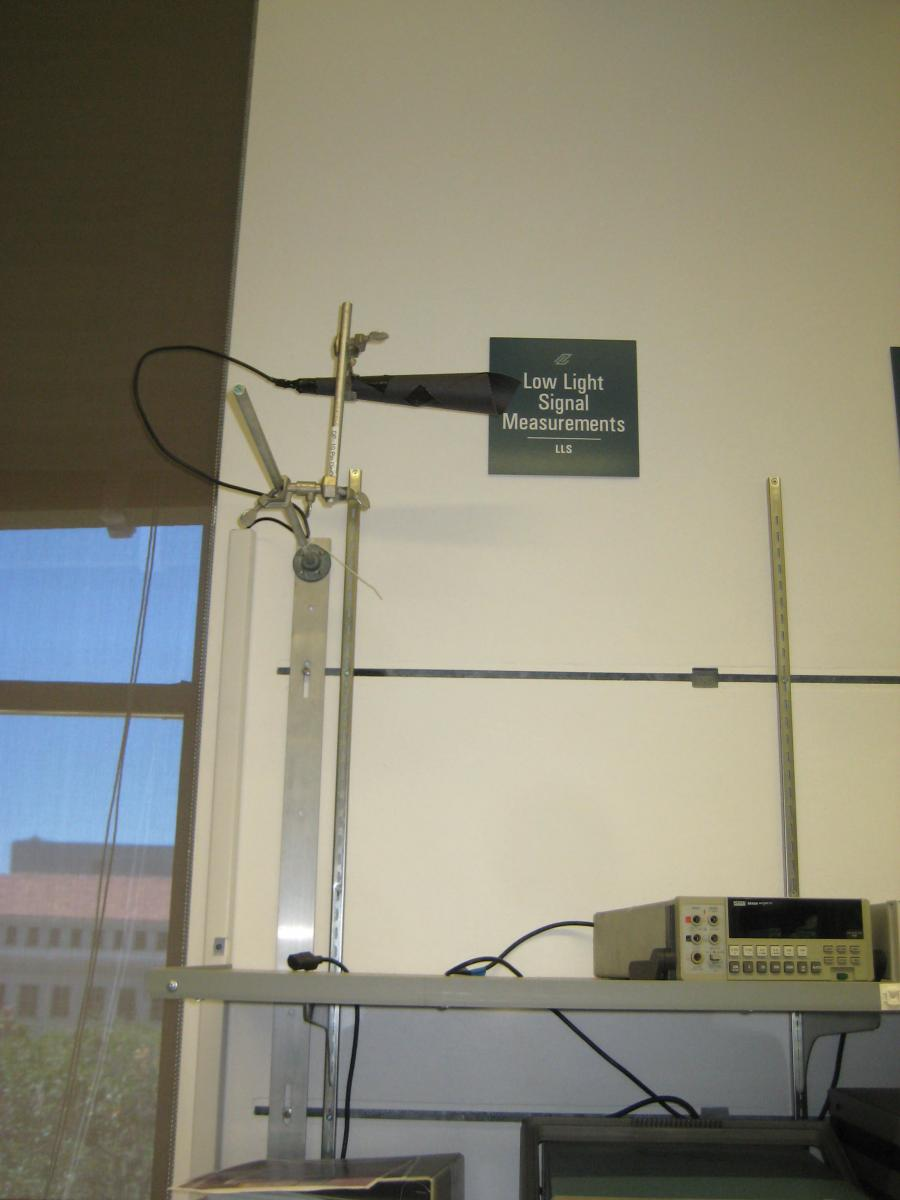
\includegraphics[width=\linewidth,keepaspectratio]{images/IMG_4091.JPG}}
  \caption{Low Light detector \\ \href{http://experimentationlab.berkeley.edu/sites/default/files/IMG_4091.JPG}{Click here to see larger picture}}
  \label{fig:IMG_4091.jpg}
\endminipage\hfill
\minipage[t]{0.466\linewidth}
  \href{http://experimentationlab.berkeley.edu/sites/default/files/images/LLS-Source_3439.jpg}{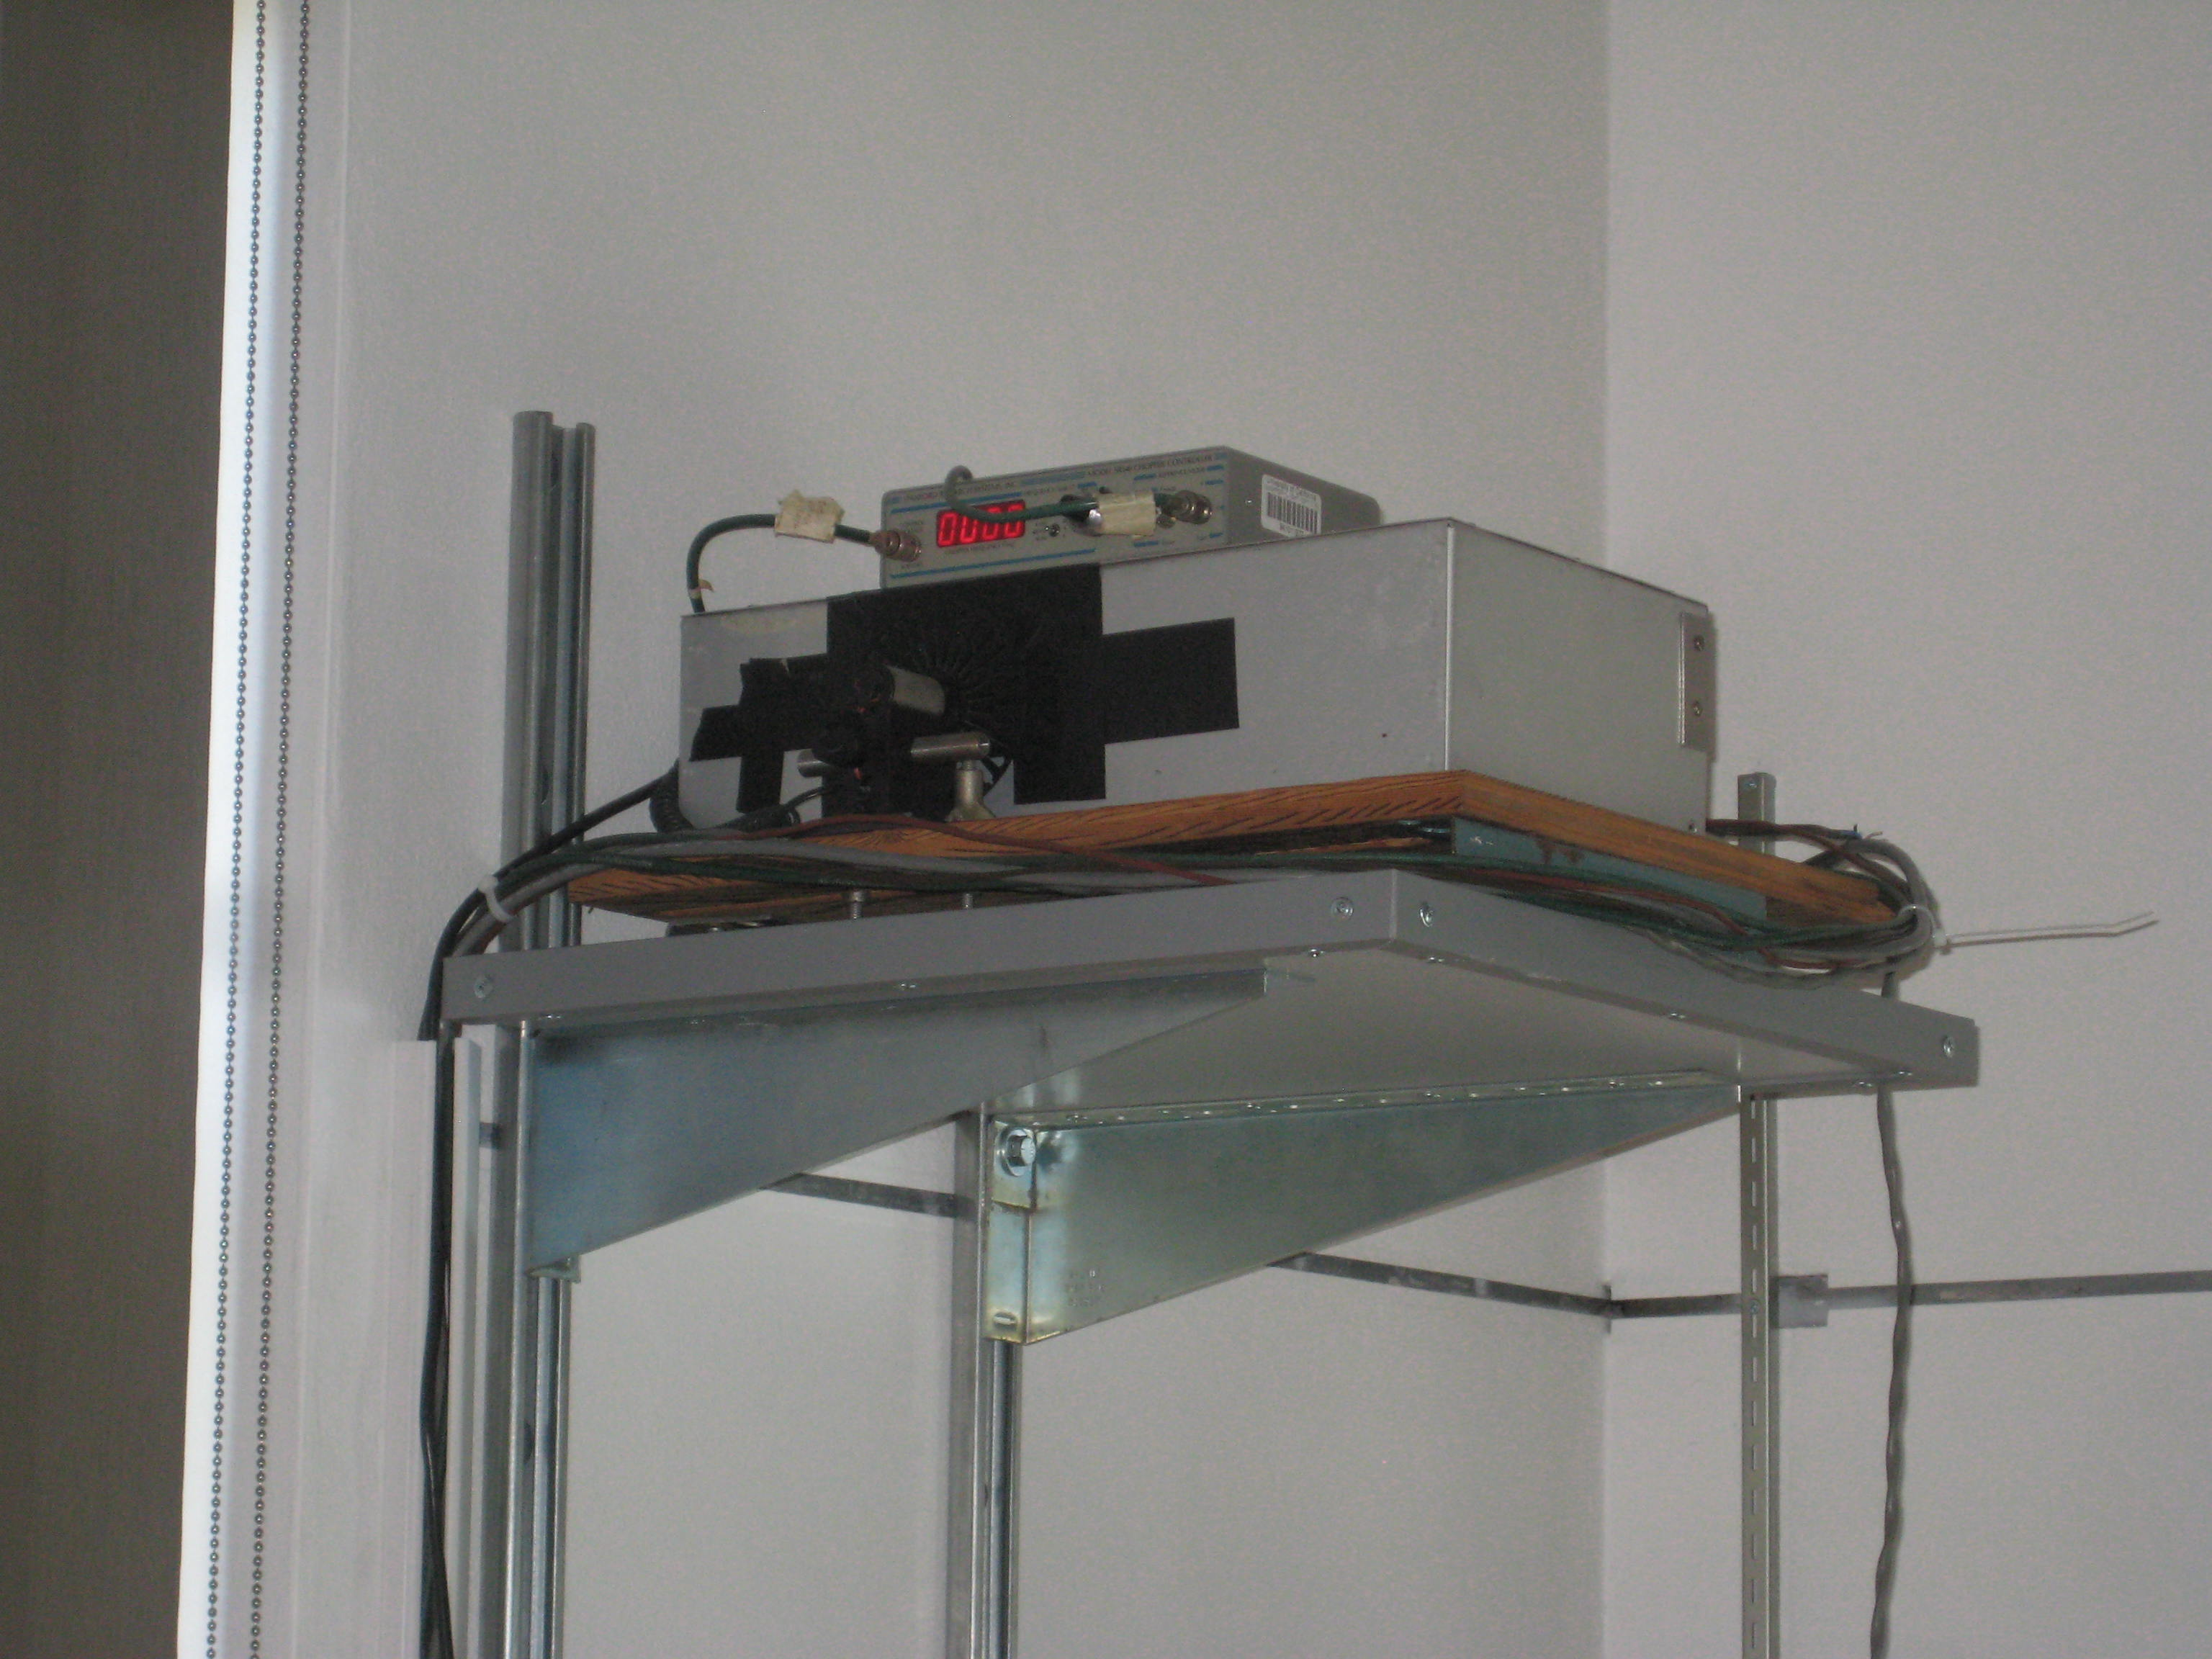
\includegraphics[width=\linewidth,keepaspectratio]{images/LLS-Source_3439.jpg}}
  \caption{Low Light Diode \& Chopper source box on NW wall \\
  \href{http://experimentationlab.berkeley.edu/sites/default/files/images/LLS-Source_3439.jpg}{Click here to see larger picture}}
  \label{fig:LLS-Source_3439.jpg}
\endminipage\hfill
\minipage[t]{0.262\linewidth}
  \href{http://experimentationlab.berkeley.edu/sites/default/files/IMG_4088.JPG}{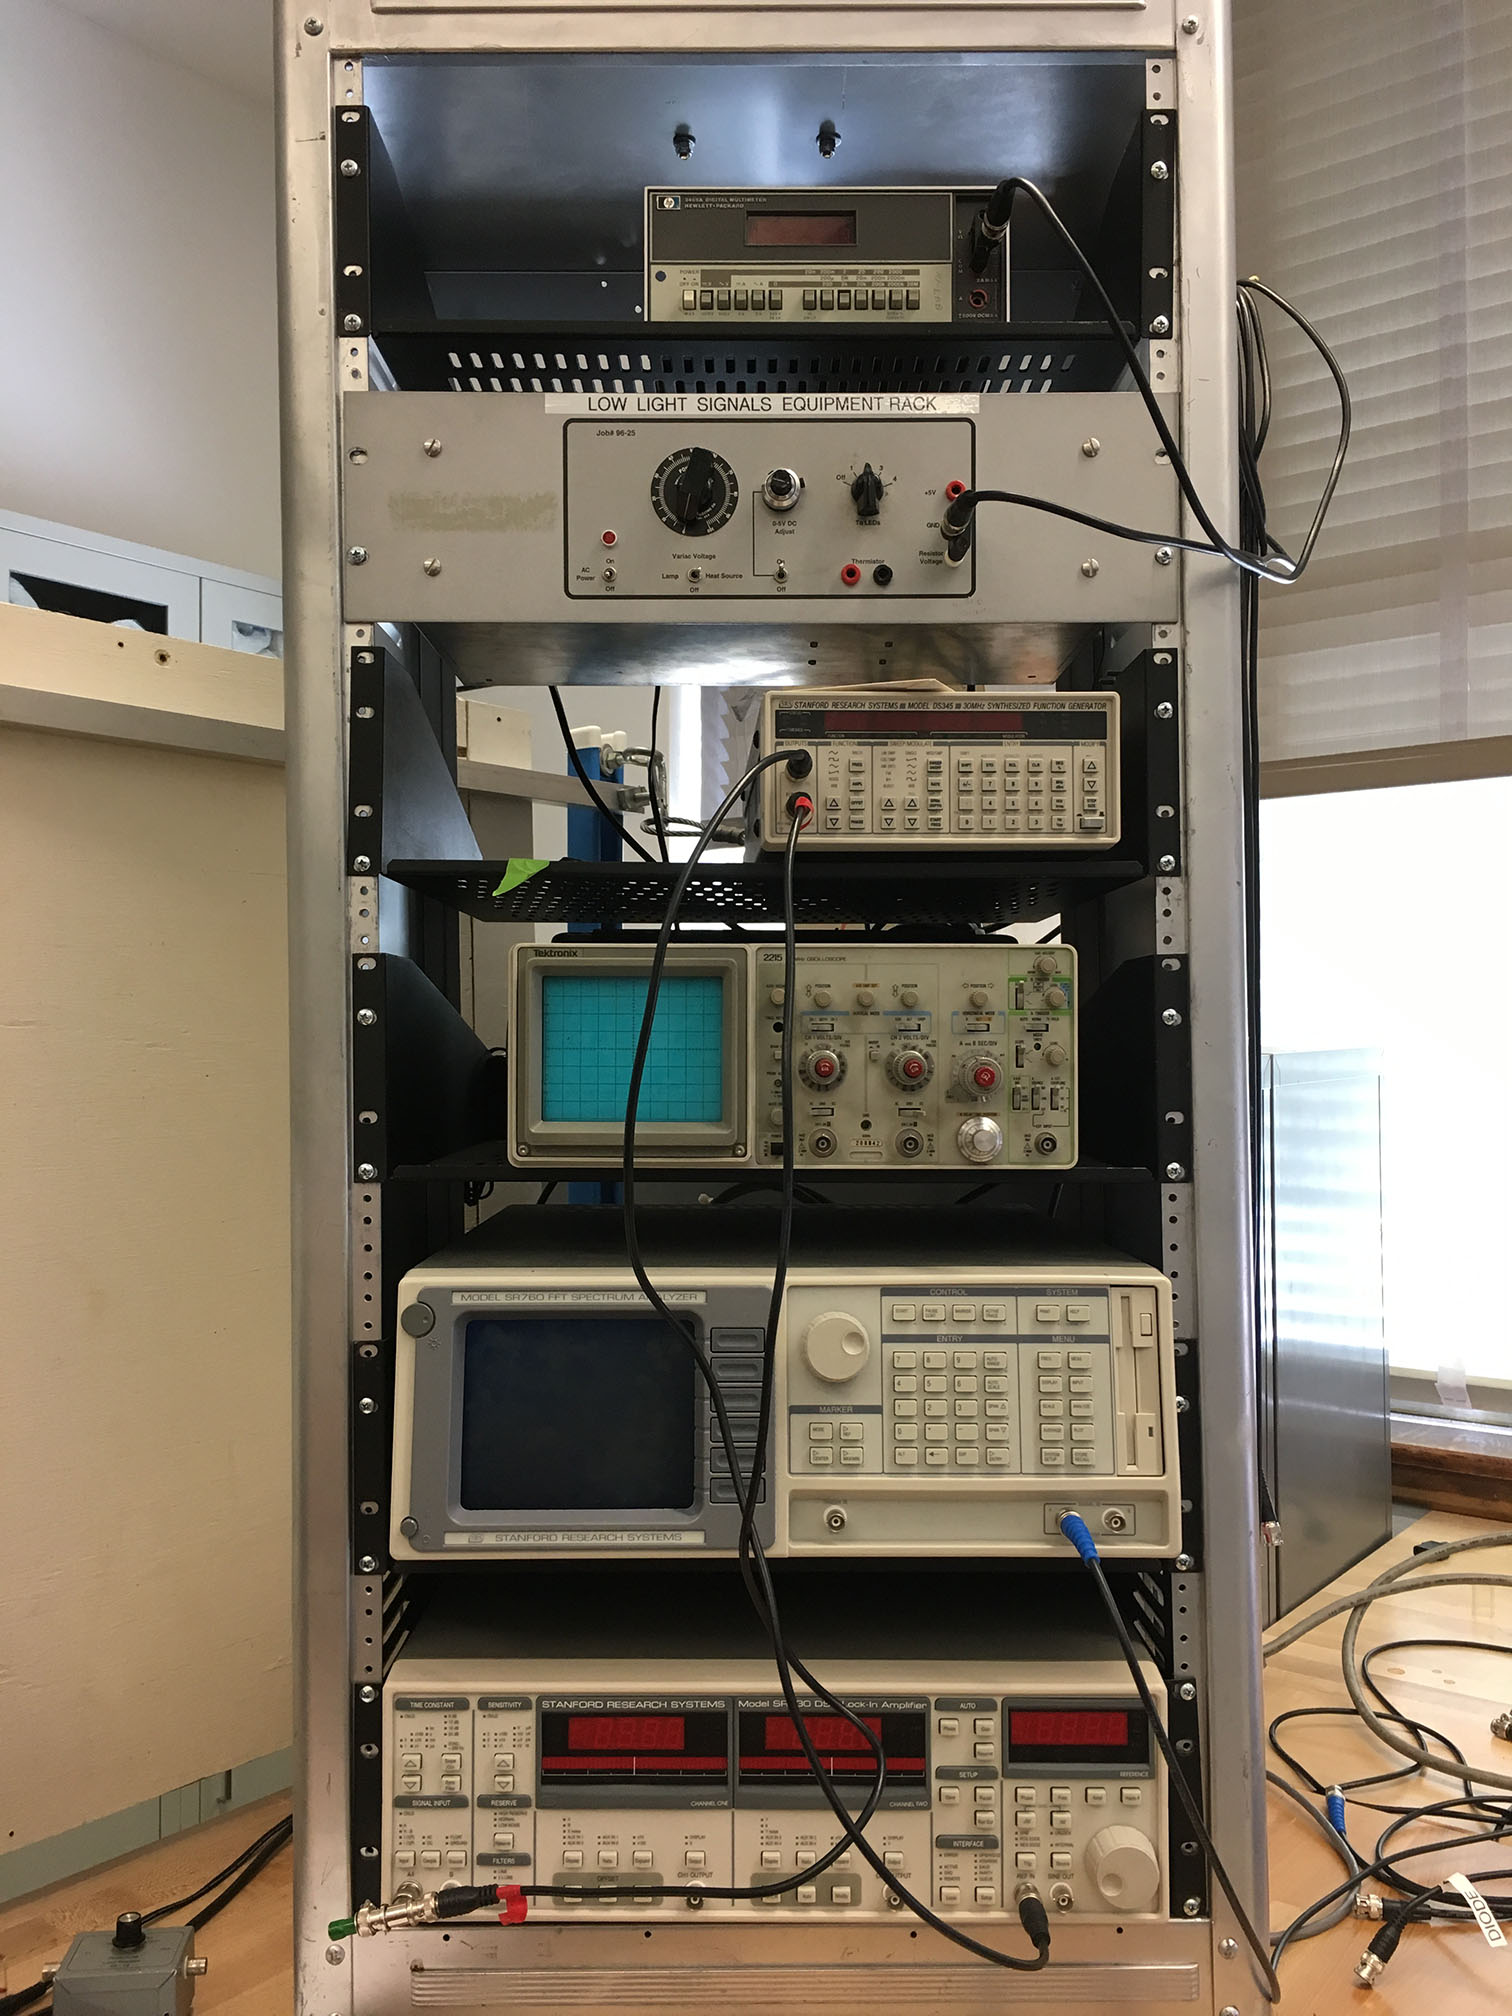
\includegraphics[width=\linewidth,keepaspectratio]{images/IMG_4088.JPG}}
  \caption{Low Light equipment rack \\ \href{http://experimentationlab.berkeley.edu/sites/default/files/IMG_4088.JPG}{Click here to see larger picture}}
  \label{fig:PigCollimator}
\endminipage
\end{figure}




\section{Before the 1st Day of Lab}

\textbf{Complete the following before your experiment's scheduled start date:}

\begin{enumerate}
    \item \emph{\textbf{Note: In order to view the private Youtube videos hosted by the university, you must be signed into your berkeley.edu Google account.}}\\
    View the two videos \href{http://youtu.be/X4XQ1jcMuoI}{\textbf{Low Light Signal Measurements}} and the \href{http://youtu.be/lQKLakISoBA}{\textbf{Light Sources and Detectors}}.

    \item Check points are examination points that are placed in this lab where you must STOP and call a GSI or professor to make sure you understand what's expected. There could  be multiple check points throughout your lab so make sure you don't skip them since there is a \href{http://experimentationlab.berkeley.edu/llscheckpoints}{\textbf{sign off sheet}} that must be turned in with your lab report. There are 5 Checkpoints in this lab.

    \item Print and fill out the \href{http://experimentationlab.berkeley.edu/LLSPreLab}{\textbf{LLS Pre Lab and Evaluation}} sheets. The Pre-Lab must be printed separately. Print it out, fill it out, turn in  your answers  with the report. Discuss the experiment and pre-lab questions with any faculty member or GSI and get it signed off by that faculty member or GSI. Turn in the signed pre-lab sheet with your lab report.

    \item Last day of the experiment please fill out the \href{\ExperimentEvaluation}{\textbf{Experiment Evaluation}}

\end{enumerate}

\noindent\textbf{Suggested Reading:}

\begin{enumerate}
    \item J. Moore, C. Davis, M. Coplan, and S. Greer, \href{http://physics111.lib.berkeley.edu/Physics111/Reprints/Apparatus\%20Book/Building-Scientific-Apparatus--Moore.pdf}{\textbf{Building Scientific Apparatus}} (Fourth ed.), Cambridge University Press, 2009.

    \item R. Ramirez, ``\href{http://physics111.lib.berkeley.edu/Physics111/Reprints/LLS/01-The\_FFT.pdf}{\textbf{The FFT: Fundamentals and Concepts}}''; Prentice-Hall, 1985, pp. 3-16 \& 115-123.

    \item E. Brigham, ``\href{http://physics111.lib.berkeley.edu/Physics111/Reprints/LLS/02-The\_Fast\_Fourier\_Transform.pdf}{\textbf{The Fast Fourier Transform}}''; Prentice-Hall, 1974, pp. 24-27.

    \item \href{http://physics111.lib.berkeley.edu/Physics111/Reprints/LLS/03-LowLight\_FFT\_Demo.pdf}{\textbf{Introduction to Low Light FFT Demo}}

    \item About Lock-In Amplifiers: Application Note \# 3” \href{http://physics111.lib.berkeley.edu/Physics111/Reprints/LLS/About-Lock-Ins.pdf}{\textbf{About Lock-ins}}

    \item Perkin Elmer Instruments. ``What is a Lock-In Amplifier?: Technical Note TN 1000'' \href{http://physics111.lib.berkeley.edu/Physics111/Reprints/LLS/Lock-in-Amp.pdf}{\textbf{Lock-in Amp}}

\end{enumerate}

\noindent More \hyperref[sec:References]{References}

[\href{\LabReprints}{\textbf{Physics 111 Library Site}}]

You should keep a laboratory notebook. The notebook should contain a detailed record of everything that was done and how/why it was done, as well as all of the data and analysis, also with plenty of how/why entries. This will aid you when you write your report.

\section{Objectives}

\begin{itemize}
    \item Learn what real experimental physics is about

    \item Learn the synergy between experimental and theoretical work

    \item Learn to use pieces of equipment that are commonly used in research

    \item Learn how measurements are performed, analyzed, and interpreted.

    \item Learn how to present your work and results

    \item Learn problem solving strategies

    \item Learn how to manage and organize your time

\end{itemize}

\section{Introduction}

The main goal of this lab is to learn about techniques for low-signal measurement and the noise sources that degrade them. You will do this by measuring the power emitted by an LED from across the room with a variety of noise sources present, including the room lights and the sun. The technique you will use is the time-honored chopper-wheel/lock-in amplifier combination.

The first section of this lab, \href{http://http://experimentationlab.berkeley.edu/IntroductiontoEquipment}{\textbf{Introduction to Equipment (LLS)}}, is composed of several ``mini-experiments'' designed to introduce you to some fancy measuring devices, generously donated to the 111 Labs by Stanford Research Systems. These experiments may seem pointless and boring, but by doing them, you will become familiar with the basic workings of the equipment, techniques for learning to use unfamiliar equipment (the most important), and other odds-and-ends stuff (e.g. different conventional units such as dBV, V/${\sqrt{\textrm{Hz}}}$,etc.). It's easy to be intimidated by all the buttons and flashy bits-but don't be. Just take your time and relax. It's really not that difficult.

In the second section, \href{http://experimentationlab.berkeley.edu/IntroductiontoNoise}{\textbf{Introduction to Noise}}, you will learn about some of the noise sources (both intrinsic and external) that hamper experimental measurements. Knowledge of things such as Johnson noise and Shot noise are very important if you plan to make low-level measurements. Knowing the limitations of measurements is an important part of experimental design. Again, you will perform several ``mini-experiments'' to acquaint yourself with noise. These range from being purely qualitative observations (e.g. looking at the $ \frac{1}{f} $noise spectrum across your fingers) to being purely quantitative (e.g. measuring the Johnson noise across numerous resistors and comparing your measurements to theoretical predictions).

It is in the third section, \href{http://experimentationlab.berkeley.edu/LightSignal}{\textbf{Measuring the Light Signal from a Diode}},that you will pull everything together and actually will measure the power output of an LED. By applying your knowledge of noise sources, you should be able to select the proper settings on the equipment so as to provide the best measurement possible. You will also look at the uncertainty in your measurements and account for them.

\subsection{A Note About Typographical Conventions in This Lab}

This lab uses several typographical conventions to help make the procedures clearer. Some of them are as follows:

\begin{enumerate}
    \item {[ STUFF ]} (text written in a special font and bracketed) usually refers to a particular button on the equipment

    \item STUFF (text not bracketed) usually refers to other parts or settings on the equipment or software interfaces.

\end{enumerate}

\textbf{Question?} written in bold type is a question for you to answer in your lab write-up.

\section{Apparatus and Equipment}

\begin{enumerate}
    \item \href{http://physics111.lib.berkeley.edu/Physics111/Reprints/LLS/11-HP3465A.pdf}{\textbf{HP 3465A DMM}}

    \item \href{http://physics111.lib.berkeley.edu/Physics111/Reprints/LLS/07-SR830.pdf}{\textbf{SRS SR830}}
    
    \item \href{http://physics111.lib.berkeley.edu/Physics111/Reprints/LLS/HM303-6_engl.pdf}{\textbf{HM303-6}} Oscilloscope

    \item \href{http://physics111.lib.berkeley.edu/Physics111/Reprints/LLS/06-SR760.pdf}{\textbf{SRS SR760}} FFT Spectrum Analyzer

    \item \href{http://physics111.lib.berkeley.edu/Physics111/Reprints/LLS/09-DS345.pdf}{\textbf{SRS DS345}} Function Generator \href{https://youtu.be/PrM8DHFOFS0}{Click here to watch an instructional video}

    \item \href{http://physics111.lib.berkeley.edu/Physics111/Reprints/LLS/05-SR570.pdf}{\textbf{SRS SR570}} Preamplifier \href{http://experimentationlab.berkeley.edu/defaultsettings}{\textbf{default settings}}

    \item AC/DC Power Supply + Heat Source

    \item \href{http://physics111.lib.berkeley.edu/Physics111/Reprints/LLS/10-SR540.pdf}{\textbf{SRS SR540}} Optical Chopper (located in northwest corner of room by the ceiling)

    \item Diode light source (located under the optical chopper)

    \item Light Detector (located at top of lab station)

\end{enumerate}

\section{The SR760 FFT Spectrum Analyzer}

Before you continue further, you should first read the \emph{Analyzer Basics} and \emph{Operation} sections of the \emph{SR760 FFT Spectrum Analyzer Operating Manual and Programming Reference}.

\subsection{Experiment I}

You will use a function generator to provide an input signal to the SR760 in order to get a feeling for how the SR760 and the function generator work. By using well-defined input signals, you can get a better feeling for how the FFT treats not-so-well defined signals. You will experiment with sine, triangle, and square wave input signals.

\begin{enumerate}
    \item Hold down the back arrow key, [$\leftarrow$], and turn on the SR760. This puts the SR760 in the default settings.

    \item Connect the output of the Function Generator to Signal In A of the SR760 with a tee and a 50 ohm terminator. Any value other than 50 ohms changes the calibrations of the SR760 internal parameters.

    \item Start with a sine wave input signal, say a 0.2 $V_\text{pp}$ ($-$20 dBV according to the SR760 units convention) at 400 Hz sine wave. The procedure for setting these values is as follows:
    \begin{itemize}
        \item To set the DS345 Digital Function Generator:
        \begin{enumerate}
            \item Turn it on.

            \item Press the up/down arrow keys [$\triangle$] [$\nabla$] by the BNC FUNCTION OUTPUT until the sine waveform is highlighted in green. To select another type of waveform output, you just press the [$\triangle$] [$\nabla$] arrow keys until the desired waveform is highlighted in green.

            \item To set the frequency of the sine wave,
            \begin{enumerate}
                \item Press the [ FREQ ] button.

                \item Enter a new frequency using the number pad and set it by pressing the appropriate units key-e.g. the [ Hz/$V_\text{pp}$ ] key.

            \end{enumerate}

            \item To set the amplitude of the output waveform,
            \begin{enumerate}
                \item Press the [ AMPL ] button.

                \item Enter the desired amplitude using the number pad and set it by pressing the appropriate units key-e.g. the [ Hz/$V_\text{pp}$ ] key. Note the various choices you have.

            \end{enumerate}

            \item You should check that everything is working properly using a scope, if one is available.

        \end{enumerate}

    \end{itemize}

    \item Now we need to make some adjustments on the SR760 to get a useful display. You want to look at the Fourier decomposition of signals in a small range that includes the signal of 400 Hz and several of its harmonics (multiples of 400 Hz). To do this, set the START FREQUENCY to 0 Hz and the SPAN to 1.56 kHz. These settings say that the range of frequencies you want to examine is from 0 to 1.56 kHz. If you don't already know how to do that, follow the instructions below.
    \begin{enumerate}
        \item To set the Start Frequency
        \begin{enumerate}
            \item Press the [ FREQ ] button in the MENU pad section on the front of the SR760

            \item Press the [ START FREQ ] soft key. A soft key is a button whose meaning changes, depending on which MENU key was pressed immediately before. All hand-held calculators have soft keys, for example. On the SR760, they're lined up at the right of the screen.

            \item Press 0 on the ENTRY pad. New menu shows up on the screen with choice of [ mHz ], [ Hz ], [ kHz ], and [ escape ]. Press the [ Hz ] soft key.

        \end{enumerate}

        \item To set the Span
        \begin{enumerate}
            \item Press the [ SPAN$\triangle$ ] / [ SPAN$\nabla$ ] keys by the number pad until the appropriate span is set \emph{OR}

            \item After pressing the [ FREQ. ] button, press [ SPAN ] soft key and turn the SPIN KNOB (the dial) until the span is 1.56 kHz. Note that 100kHz is a maximum value.

        \end{enumerate}

    \end{enumerate}

    \item Now it's time to see what the SR760 is doing to the sine wave, so look at the display on the SR760. You should see a large peak at 400 Hz, the frequency of the input sine wave. Be quantitative and get a measurement to see if its frequency and amplitude are correct. To do so do the following:
    \begin{enumerate}
        \item Press the [ MEAS. ] button in the MENU section. This will tell the SR760 that you want to measure something. The SR760 then re-defines the soft keys and the operation of the SPIN KNOB.

        \item Turn the SPIN KNOB until the marker (the little black square on the screen) is at the top of the main peak. Look at the top row center on the screen. It should read \emph{$-$20 dBV}. Does it? Remember that the instrument can display a signal in different units, such as Volts pp, Volts rms, decibel Volts (dBV = 20 log $V$), etc. Acoustical and electrical engineers like to use decibels, while most of us like to use just plain volts. To familiarize yourself with these different units, go to the [ MEAS ] $\rightarrow$ [ UNITS ] menu and try out the different settings.

    \end{enumerate}

    \item You may notice that the peak does not lie exactly at 400 Hz, (top row left) but at some close frequency, such as 398.44 Hz. \textbf{If so, is this a fault of the function generator or of the SR760?} Experiment with different SPAN settings of the FFT, to measure the frequency more accurately.

    \item The DS345 is a good function generator. However, you may notice that there are also smaller amplitude sine waves whose frequencies are multiples of the 400 Hz fundamental sinusoid. These are called harmonics. The second harmonic is twice the frequency of the first harmonic or fundamental frequency sine wave. If you don't see any, try using the \emph{Linear Averaging (RMS)} feature and perhaps increase the SPAN (don't spend too much time doing this-they may not be readily visible). The \emph{Linear Averaging} feature takes many transforms and linearly averages them. See the SR760 operating manual for instructions on its use or just poke a few buttons. You might start with the [ AVERAGE ] button. If you have the opportunity, you might use an analog function generator from \textbf{BSC} to observe higher harmonics.
    \begin{enumerate}
        \item \textbf{If you see higher harmonics}, \textbf{does that mean the signal generator is not producing a perfect sine wave?}

        \item \textbf{If you don't see any higher harmonics, does that mean the signal generator is producing a perfect sine wave? Explain.}

    \end{enumerate}

    \item Now experiment using different types of input waveforms. Look at the Fourier spectra of triangular and square waves. Note what you see on the screen for each waveform. \textbf{Are they what you expect mathematically? Explain.}

\end{enumerate}

\subsection{Optional Exercise for the FFT:}

\emph{If you felt comfortable with the previous experiment, then skip to Experiment II. Otherwise, you can solidify your understanding of the FFT with the following exercise.}

\noindent\textbf{Examine a sine wave in the time domain with a oscilloscope and the frequency domain with the FFT}

\begin{enumerate}
    \item Link the generator's function output to both the FFT input and the scope input. \emph{Remember a 50-Ohm terminator on the end of each wire connecting to scope and FFT!}

    \item Configure the function generator to produce a sine wave with a 0.5 $V_\text{pp}$ amplitude and a frequency of 4300 Hz. Using the scope make sure everything is working correctly. Procedure is as follows:
    \begin{enumerate}
        \item Turn on the SRS DS345 Function generator

        \item \emph{To select a sine wave output:} Press the up/down arrow keys, [$\triangle$] [$\nabla$], by the BNC FUNCTION OUTPUT until the sine waveform is highlighted in green. To select another type of waveform output, you just press the [$\triangle$] [$\nabla$] arrow keys until the desired waveform is highlighted in green.

        \item \emph{To set the frequency of the output}:
        \begin{enumerate}
            \item Press the [ FREQ ] button

            \item Type 4300 using the number pad

            \item Set the new frequency by pressing the [ Hz/$V_\text{pp}$ ] button

        \end{enumerate}

        \item \emph{To set the amplitude:}
        \begin{enumerate}
            \item Press the [ AMPL ] button

            \item Type 0.5 using the key pad

            \item Set the new amplitude by pressing the [ Hz/$V_\text{pp}$ ] button

        \end{enumerate}

        \item \emph{In General}: To select a frequency, amplitude, offset, or phase of the output wave:
        \begin{enumerate}
            \item First press one of those 4 buttons in the FUNCTION area on the front panel

            \item Enter the desired value with the keypad.

            \item To make the new setting take effect press the appropriate units key in the right column of the ENTRY area.

        \end{enumerate}

    \end{enumerate}

    \item We want to set the SPAN of SR760 to 6.25 kHz and switch the display to linear magnitude:
    \begin{enumerate}
        \item To turn on the SR760 hold down the back-arrow key, [$\leftarrow$], on the SR760 FFT ENTRY pad and turn on the power. You should hold down the back-arrow key until all of the internal tests have completed and the FFT has started taking data. This starts the FFT in default mode. Note: occasionally you may see the FFT freeze and display the message: ``Calibrating Offset.'' This is normal and nothing to worry about. Just wait until it's done before continuing.

        \item To set the SPAN
        \begin{enumerate}
            \item Press the [ FREQ ] button in the MENU area.

            \item Press the top-most soft key near the monitor (the one corresponding to the span). 100 kHz should be highlighted in green. Note: if you pressed the wrong soft key, just hit the [ FREQ ] button in the MENU area and try again.

            \item Turn the SPIN KNOB counter clockwise until the highlighted number reads 6.25 kHz. The span has now been set to 6.25 kHz.

        \end{enumerate}

        \item To set the display mode to Linear Magnitude:
        \begin{enumerate}
            \item Press the [ MEAS ] key in the MENU area.

            \item Press the soft key second from the top (it corresponds to DISPLAY). Again, if you hit the wrong soft key, just press the [ MEAS ] key in the MENU area and try again.

            \item You should now see the following choices on the screen: [ Log Mag. ], [ Lin Mag ], [ Real Part ], [ Imag. Part ], [ Phase ]. Press the soft key corresponding to [ Lin Mag ]. (the second from the top). If you make a mistake, just press the correct soft key. The FFT should now be displaying the linear magnitude of the Fourier components instead of their Log magnitudes. Notice how all the noise disappears (we will come back to this later).

            \item Now press the [ AUTO SCALE ] button located in the right column of buttons in the ENTRY section. This will re-scale display. You should now see a single peak on the FFT screen.

        \end{enumerate}

    \end{enumerate}

    \item If everything is working properly, you are now ready to examine a single sine wave in the time and frequency domain.
    \begin{enumerate}
        \item Look at the sine wave on the oscilloscope. What you should see is a sine wave with an amplitude of 250 mV (0.5 $V_\text{pp}$) and a frequency of 4.3 kHz. If the amplitude is not what you would expect it to be, make sure you have a 50-Ohm terminator. As you know the scope is plotting the voltage output of the function generator as a function of time. It is representing the function generator's output in the ``time domain.''

        \item Now look at the FFT. First measure the position and amplitude of the peak you should be seeing. To do this:
        \begin{enumerate}
            \item Press the [ MEAS ] button. This will change the SPIN KNOB's function.

            \item Dial the SPIN KNOB until the cursor on the screen locks to the peak. This should happen when the peak is between the two vertical dashed lines.

            \item Read the location (frequency and amplitude) of the cursor in the upper-left hand corner of the screen.

            \item You should find that the peak is located around 4.3 kHz and has an amplitude of about 250 mV. Note that the values may not be exactly 4.3 kHz and 250 mV. The reasons for this will be discussed later in the lab.

        \end{enumerate}

        \item A single peak on the FFT display corresponds to a single sine wave with a frequency and amplitude given by the height and location of the peak.

        \item Now vary the frequency of the sine wave and watch what happens on the scope and the FFT.
        \begin{enumerate}
            \item Vary the frequency:
            \begin{enumerate}
                \item On the DS345 Function generator, press the [ FREQ ] button. You should now see that the sine wave has a frequency of 4.3 kHz (the green FREQ should be lit up under the readout).

                \item Now press the [ STEP SIZE ] button in the MODIFY section. Now both FREQ and STEP should be lit up in green under the display.

                \item Using the [$\triangle$] [$\nabla$] arrows directly above the [ STEP SIZE ] button, adjust the STEP SIZE to read 100.000. This will determine how much the frequency will change when you press the [$\triangle$] [$\nabla$] keys later.

                \item Now press the [ FREQ ] or [ STEP SIZE ] button. The screen should read 4300 Hz and only FREQ should be lit up in green under the display.

                \item Now press the [$\triangle$] [$\nabla$] keys in the MODIFY section. The frequency reading should change in steps of 100 Hz since you have just adjusted the STEP SIZE to 100 Hz.

                \item Watch the peak move back and forth on the FFT.

            \end{enumerate}

        \end{enumerate}

        \item Now vary the amplitude of the sine wave and watch what happens.
        \begin{enumerate}
            \item Press the [ AMPL ] button on the DS345 Function Generator. AMPL should be lit up in green under the main display which should read 0.500 $V_\text{pp}$.

            \item Now press the [ STEP SIZE ] button in the MODIFY section (STEP should light up).

            \item Using the keypad in the ENTRY section, enter .05 and set the value by pressing the [ Hz/$V_\text{pp}$ ] key.

            \item Press either the [ AMPL ] or [ STEP SIZE ] buttons

            \item Adjust the amplitude with the [$\triangle$] [$\nabla$] keys in the MODIFY section.

            \item Watch how the height of the peak changes in correspondence with the change in amplitude.

        \end{enumerate}

    \end{enumerate}

    \item Now change the input waveform to a square wave and a triangle wave.

\end{enumerate}

You should now have a fairly good idea as to how the FFT treats a pure sine wave and how to take simple measurements.

\section{Introduction To Noise}

Noise plagues everything. Sometimes it can be so small compared to the signal of interest that it doesn't matter. This is not usually the case). Often different potential sources of noise must be taken account of so that noise can be avoided or even eliminated through experimental design or measuring techniques. In this section, you will learn about and explore the following types of noise:

\subsection{Intrinsic (Random) Noise Sources}

\begin{enumerate}
    \item \textbf{$ \frac{1}{f} $ Noise: Higher noise amplitude at low frequencies. This noise makes low frequency measurements more difficult. Its origin is poorly understood. You should learn to recognize it and its effects on measurements.}

    \item \textbf{Capacitive Coupling Noise:} AC voltages from nearby electronics create stray capacitive effects. Careful design can nearly eliminate capacitive noise.

    \item \textbf{Microphonic Noise:} Mechanical vibrations/movements affect the electronic components. Shaking a cable = microphonic noise.

    \item \textbf{Shot Noise:} Non-uniformity in the electric current due to the quantization of charge carriers. Since Shot Noise depends on frequency bandwidth, the Lock-in will be able to eliminate most of this noise.

    \item \textbf{Input Noise of Instruments:} Aggregate noises of many components in an instrument. Proportional to square root of bandwidth.

    \item \textbf{Johnson Noise:} Voltage noise across a resistor due to thermal fluctuations in the electron density. Called ``white noise'' because it's the same for all frequencies.

\end{enumerate}

\subsection{Before you begin this section}

Read the blurb on different noise sources in the SR830 Lock-In Operating Manual (starting on page 3-21).

\subsection{Other references}

\begin{enumerate}
    \item Moore, Davis and Coplan, \emph{Building Scientific Apparatus}. It is a little more detailed than the SR830 Operating manual; a good reference for just about anything, not too advanced.

    \item M. J. Buckingham, \emph{Noise in Electronic devices and Systems} . Its treatment is exhaustive and rather advanced. Unless you groove on ugly math, you'll probably only find the semi-qualitative introductions useful.

    \item Kogan, \emph{Electronic Noise and Fluctuations in Solids}. It's also quite advanced--yet filled with all sorts of good information.

\end{enumerate}

\section{SR830 Lock-in Amplifier}

The first few sections in chapter 3 of the manual are useful towards understanding how the lock-in amplifier works.

One crucial piece of information I believe is essential towards understanding the amplifier is understanding what exactly it is measuring. This blurb below is taken from the operating manual from section 3-3:

``What does the SR830 measure? The SR830 multiplies the signal by a pure sine wave at the reference frequency. All components of the input signal are multiplied by the reference simultaneously. Mathematically speaking, sine waves of differing frequencies are orthogonal, i.e. the average of the product of two sine waves is zero unless the frequencies are EXACTLY the same. In the SR830, the product of this multiplication yields a DC output signal proportional to the component of the signal whose frequency is exactly locked to the reference frequency. The low pass filter which follows the multiplier provides the averaging which removes the products of the reference with components at all other frequencies.''

It goes on to further explain the physical and mathematical process behind the Lock-in Amplifier and is a good place to start reading.

\subsection{Experiment II}

This experiment is very similar to the previous one. In order for you to get a feeling for how the lock-in works, you're going to feed it a sine wave of known frequency and amplitude. Along the way you'll push some buttons and take some measurements.

\begin{enumerate}
    \item Turn on the SR830 while holding down the interface setup key (the ON-OFF switch is on the back by the power cord). Release the key after the instrument starts beeping. All the defaults will then be set. Turn on the DS345 Function Generator.

    \item Feed the Lock-In a sine wave with a frequency of about 1 kHz and 2 $V_\text{pp}$:
    \begin{enumerate}
        \item Connect the FUNCTION output of the DS345 to INPUT A/I of the SR830 (remember the 50-Ohm terminator!).

        \item Set the DS345 so that it produces a 2 $V_\text{pp}$ sine wave at a frequency somewhere around 1 kHz. To set the frequency press [ FREQ ], [ 1 ], [ kHz/$V_\text{rms}$ ]. To set the 2 $V_\text{pp}$ sine wave press [ AMPL ], [ 2 ], [ Hz/$V_\text{pp}$ ]. In the FUNCTION section of DS345 press the [$\triangle$] [$\nabla$] keys until the sine wave function is lit. If you want to try out different waveforms at a later time, keep these things in mind:
        \begin{enumerate}
            \item To avoid damaging the SR830, make sure the input voltage is less than 50 V.

            \item To avoid overloading the Lock-In, keep the input voltage less than 1 $V_\text{rms}$.

        \end{enumerate}

        \item To provide a reference signal with the same frequency as the sine wave for the SR830, Connect the SYNC output of the DS345 to the REF IN of the SR830 (you don't need a 50-Ohm terminator here).

    \end{enumerate}

    \item Now make sure that the settings are all right.
    \begin{enumerate}
        \item You'll probably want to measure the magnitude of the signal, so set the CHANNEL ONE DISPLAY of SR830 to \emph{R} (magnitude of signal) and the CHANNEL TWO DISPLAY of SR830 to $\theta$ (phase angle between the input signal and reference signal). To adjust these, hit the corresponding [ DISPLAY ] buttons.

        \item Verify that the reference frequency is the same as the input frequency by pressing the [ FREQ ] button under the REFERENCE WINDOW (you should see the reference frequency displayed in the window above the SPIN KNOB). If it is not, press the [ SOURCE ] button by the SPIN KNOB so that the reference signal is switched off of INTERNAL (the SR830 also has its own internal oscillator you can use if a reference signal is not available).

        \item Adjust the SENSITIVITY to fit the level of the signals you are going to measure. The term ``sensitivity'' as used here by the instrument manufacturer means ``set the detector to the maximum value of the quantity that you want to measure.'' For examples, if the signal is going to be 1 volt max, set the sensitivity to 1 volt. This is considered a large sensitivity. If the largest signal will be 25 mV, set the sensitivity to 25 mV. This is considered to be a small sensitivity! When the ``sensitivity'' is smaller than the signal, CHANNEL ONE displays an overload warning. Alternatively, you may not have the resolution you want. To adjust the SENSITIVITY, press the [$\triangle$] [$\nabla$] arrow buttons in the SENSITIVITY section of the SR830 until an appropriate value is attained. \textbf{If your signal is a .2 $V_\text{pp}$ sine wave, your sensitivity should be greater than 71 mV. Why? Remember that the SR830 displays rms amplitudes.}

        \item Learn about the TIME CONSTANT\emph{ }from the Lock-In manual. For a signal with constant amplitude, a general rule is that the larger the TIME CONSTANT, the more stable the measurement. \textbf{Why? }Experiment with different time constants (remember that it takes 5 time constants for the signal to settle to 99\% of its actual value). \textbf{Would you want to maximize the TIME CONSTANT if you were trying to track a signal whose amplitude was varying? What would you have to take into consideration?}

        \item Does the output roughly agree with what it should be? (Remember, the reading is in $V_\text{rms}$ \emph{not} $V_\text{peak amplitude}$.). \textbf{If the reading is off by a few millivolts, why?}

    \end{enumerate}

    \item Now change the input waveform to a 2 $V_\text{pp}$ square wave. To do that press the [$\triangle$] [$\nabla$] keys in the function section of DS345 until the square wave is lit. The SR830 Basics section of the manufacturer's manual states that you will measure not the amplitude of the square wave, but the amplitude of its fundamental Fourier component (or the amplitude of the Fourier component at the reference frequency). It also says that a 2 $V_\text{pp}$ square wave of frequency $\omega$ can be written as 1.273sin[$\omega t$] + 0.4244sin[3$\omega t$] + 0.2546sin[5$\omega t$] + ...

\end{enumerate}

The manual goes on to say that the SR830 locked to angular frequency $\omega$ will ``...single out the first component''. The measured signal will be 1.273sin[$\omega t$], not the 2$V_\text{pp}$ that you'd measure on a scope. \textbf{What voltage do you expect the SR830 to display? Does it?} Again you may be off by a few millivolts or so. The root to this problem is probably the ``50$\Omega$'' terminator resistor. If it's not 50$\Omega$, the desired output of the function generator will not be what is input to the Lock-In. The setup basically acts like a voltage divider: the function generator has 50$\Omega$ in it, and adjusts its output voltage to terminate into 50$\Omega$. So the larger the terminating resistance, the larger the input voltage to the Lock-In. If you remove the terminator entirely, the input voltage will be nearly twice what it should (the input impedance of the Lock-In is much greater than 50$\Omega$). Experiment with different terminators. The ones in back may range anywhere from about 52$\Omega$ to 81$\Omega$.


\textbf{This is a Checkpoint: Call over a GSI and explain the difference between the $V_\text{pp}$ and the $V_\text{p}$ when dealing with the Fourier components of the square wave, why does the voltage value appear larger on the Lock-in when moving from a sine wave to a square wave of the same amplitude (Hint: Try looking up the Fourier decomposition of a square wave and the amplitude of the first component). Next, explain why the voltage of the SRS is a few millivolts off its desired value. }

\subsection{Experiment III}

Now you're going to learn to use the interface software for the Lock-In. You'll also explore the effects and the role of time constants on measurements. Basically you're going to vary the input signal amplitude and see how quickly the Lock-In can respond. Read the entire procedure before beginning.

\begin{enumerate}
    \item Use the DS345 function generator to provide the SR830 with an input sine wave: 2 $V_\text{pp}$ (we don't want to overload the SR830) with a frequency of 1 kHz or so.

    \item Set [ SLOPE/OCT ] to 6 dB on the Lock-In (by the TIME CONSTANT controls). This partially determines how ``steep'' the low-pass filter is (see \href{http://experimentationlab.berkeley.edu/node/99}{\textbf{Appendix D: the Phase Sensitive (Lock-In) Detector}}). We'll start out small (6 dB) and work our way up (24 dB).

    \item At this point, you may want to read \href{http://experimentationlab.berkeley.edu/node/97}{\textbf{Appendix B: SR830 Lock-In Interface Program}} for more detailed information about the workings of the Lock-In Interface program.

    \item Start the program \emph{LowLight SR830 Lock-In Interface} by double clicking on its icon.

    \item Set the following data-saving parameters on the interface program:
    \begin{enumerate}
        \item NUMBER OF RUNS: 1 (i.e. you'll only be taking one data run)

        \item SAVE DATA: Yes (check the box) (You will want to include a plot of the data in your write-up)

    \end{enumerate}

    \item Press [ BEGIN ]. The save window will prompt you to choose the base file path and name. Choose whatever you want (preferably to your own disk) and proceed to set the following operating parameters:
    \begin{enumerate}
        \item GPIB ADDRESS: 8 (you shouldn't have to ever change this - it's just tells the computer where it can find the SR830.)

        \item SAMPLE MODE: Best Choice

        \item TIME CONSTANT: 300 milliseconds (we will want to change that later to 1s but because of a bug in the program preventing us to chose the SPAN we have to do certain operations first). This sets the SPAN to 19s (Time Constant and Span are linked in the Best Choice Mode). Now change SAMPLE MODE to Custom and the TIME CONSTANT to 1s.

        \item SAMPLE RATE: 32 Hz (the number of data points collected per second).

    \end{enumerate}

    \item Press [ START ] (The computer should start taking data).

    \item A second or two after the program begins acquiring data, change the amplitude of the input sine wave to 0.02 $V_\text{pp}$. To do this quickly, input the new value for the amplitude on the function generator before you start the run, but wait to press the units button (i.e. [ Hz/$V_\text{pp}$] ) until you're ready (the function generator won't make any changes until everything's specified). The following \textbf{Figure \ref{fig:LLSimage013}} shows what the output of the program might look like.

\end{enumerate}


\begin{figure}[h]
    \centering
    \href{http://experimentationlab.berkeley.edu/sites/default/files/images/LLSimage013.jpg}{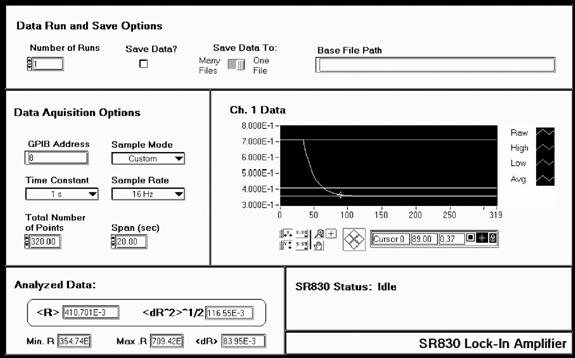
\includegraphics[width=0.6\linewidth]{images/LLSimage013.jpg}}
    \caption{The output of the program}
    \label{fig:LLSimage013}
\end{figure}

\begin{enumerate}
    \item When the program has plotted the data, you may see a typical ``RC'' decay. \textbf{From the graph, determine the time constant of the lock-in.} Hint: using the cursor feature of the Interface program. To move the cursor, use the buttons that are in the shape of a rhombus.
    \begin{itemize}
        \item Note: the data are plotted as a \emph{(signal value)} vs. \emph{(data point number)} and \textbf{not} \emph{(signal value) }vs. \emph{(time)}. However, it is easy to convert from a bin number to a time-each bin represents a time interval of 1/sample rate.
    \end{itemize}

    \item To make another data transfer you do not need to restart the program. There are two choices. One, click on the arrow in the upper left corner (note: this arrow only shows up if you have already done a transfer of the data at least once.) Another choice is to choose [ RUN ] from the OPERATE menu option.

    \item Explore different values for [ SLOPE/OCT ] for different values of the [ TIME CONSTANT]. \textbf{Do you see a pattern in the effective time constant? Is the effective time constant given by the ENBW?} (see p. 3-21 of the SR830 Basics section.)

\end{enumerate}

\subsection{Experiment IV}

This is basically an extension to Experiment III. You're going to determine how quickly you can track a signal given and what thing you'll need to take into consideration when determining the proper \emph{time constant} and \emph{[slop/oct] }settings.

\begin{enumerate}
    \item Follow the procedure for Experiment III up until number 6)

    \item Instead of using the settings in 6) of Experiment III, input the following settings:
    \begin{enumerate}
        \item GIPB ADDRESS: 8

        \item SAMPLE MODE: Best Choice

        \item TIME CONSTANT: 100 milliseconds. This sets the SPAN to 9 ms. Now, change SAMPLE MODE to Custom and TIME CONSTANT to 1s (remember we are doing this because there is a bug in the program).

        \item SAMPLE RATE: 128 Hz

    \end{enumerate}

    \item Press [ START ]

    \item Every 1/2 second or so, toggle the amplitude of the input sine wave between 2 $V_\text{pp}$ and 1 $V_\text{pp}$ (note: you only need to do this for the 9 seconds that data is being acquired).

\end{enumerate}

\textbf{This is a Checkpoint: Call over a Professor or GSI and explain where the pattern in the effective time constant is coming from. What do changes in the value of slope/oct and time constant do towards your measurement? Is the data an accurate representation of how the amplitude of input signal was changing?}

\section{The SR570 Low-Noise Current Preamplifier}

The SR570 Low-Noise Current Preamplifier, with the 1000 ohm 1\% resistor across the input terminal, converts an input current signal to a voltage signal without adding much noise (we will use the SR570 to boost the signal from the PIN10-DP Photo-diode later in the lab). The operation of the SR570 is relatively simple. The following exercises are meant to get you acquainted with the basic operation of the device. \textbf{Before continuing, you should read the following from the SR570 Operating Manual:}

\begin{enumerate}
    \item Introduction Section (p.1)

    \item Operation and Controls (Front Panel Operating Summary section (p.p. 3-6)

    \item And the Verifying Specifications section (p. 5)

\end{enumerate}

\noindent A few things to note:

\begin{enumerate}
    \item The input current should produce an output voltage of 1V or less

    \item The source used for measurements should have an impedance greater than 1/sensitivity

    \item For best performance, the SR570 should be warmed up for one hour before use

    \item \href{http://experimentationlab.berkeley.edu/defaultsettings}{\textbf{Default settings}}

\end{enumerate}

\subsection{Experiment V}

\subsubsection{A brief introduction to the workings of the SR570}

\begin{enumerate}
    \item Turn on the SR570. If we were interested in achieving the best performance using the SR570, we would let it sit and warm up for an hour at this point. However, since we are just getting an idea as to how it works, we won't concern ourselves about letting it warm up.

    \item Use a DMM to measure the current being put out by the PIN-10DP Diode (use the DC setting). (\emph{Note: the DMM will attempt to measure what it thinks to be an RMS value for the current.) The Diode is located inside a black paper cone near the ceiling towards the right of the apparatus. However, you are not expected to make your way up there, a coaxial cable runs down the wall and exits near the apparatus (it is a black coax and has a label marked ``DIODE DETECTOR''). The DMM is located on the top shelf of the shelving unit holding the equipment}

    \item Adjust the settings on the SR570 as follows:
    \begin{enumerate}
        \item FILTER TYPE: None (We won't worry about filtering the output signal, right now)

        \item GAIN MODE: Low Noise (See the operating manual for more information about gain modes.)

        \item SENSITIVITY: Roughly x100 microA/V (This is basically gain. Remember, the pre-amp converts a current to a voltage, this just specifies the inverse of the resistance. Thus, the lower the sensitivity, the higher the gain. Output on the DMM is 1 Volt or less)

        \item BIAS VOLTAGE: Off (i.e., the ``on'' position is not lit up)

        \item INPUT OFFSET: Off (i.e., the ``on'' position is not lit up)

        \item Hook up the OUTPUT of the PIN-10DP Photodiode to the INPUT of the SR570 and measure the output voltage Vout of the SR570 on the DMM. \textbf{Does the DMM Match this value? (Hint: }The PREAMPLIFIER serves to ``amplify'' your signal based on the sensitivity measurements).

    \end{enumerate}

\end{enumerate}

\subsubsection{A few notes about the Filters}

Suppose you have a signal that contains so much noise at a known frequency or range of frequencies (e.g. 60/120 Hz noise) that any amplification of it would overload either

\begin{itemize}
    \item The SR570 itself or

    \item The input of an instrument that you plan to hook up to the OUTPUT of the SR570.
\end{itemize}
It may be in your best interest to eliminate this extra noise as much as possible. That's one of the uses of the various filter options on the SR570.

If the Gain Mode is set to Low Noise, the filtering happens after the amplification. If the Gain mode is set to High Bandwidth, the filtering occurs before the amplification. However, using a high bandwidth gain has a disadvantage over the low noise gain in that it introduces more noise (see p.8 of the SR570 Operating Manual). Keeping these things in mind, which Gain setting would you use to cure the two different problems described above?

\section{1/\texorpdfstring{$f$}{f} Noise}

From \emph{Noise in Electronic Devices and Systems}

\begin{enumerate}
    \item The origin of 1/$f$ noise is poorly understood. However, you should learn to recognize it and its effects on measurements.

    \item Its spectral density (noise power /unit frequency interval) varies as 1/$f^\alpha$, where α typically varies from 0.8 to 1.4 (depending on the material) and is more or less constant over large frequency ranges.

    \item 1/$f$ noise has been observed from $10^{-6}$ Hz up to $10^6$ Hz and higher.

    \item 1/$f$ noise exists in practically all electronic devices, metal films, whiskers, liquid metals, electrolytic solutions, thermionic tubes, superconductors, and Josephson junctions. Buckingham also claims that it exists in many types of music, the measurements of the flood levels of the river Nile, the normal human heartbeat and neuro-membranes (p. 144).

    \item Other names include: current noise, excess noise, flicker noise, semiconductor noise, and pink noise (don't ask me...).

\end{enumerate}

\subsection{Experiment VI}

This experiment is mostly qualitative. You're basically going look at the 1/$f$ noise across your fingers and say, ``That's 1/$f$ noise.''

\begin{enumerate}
    \item Turn on the SR760 FFT (don't forget to press the back arrow [$\leftarrow$] button so that the SR760 resets to the default settings). We'll be using the FFT so we can verify the 1/$f^\alpha$ spectrum.

    \item Start the \emph{LowLight FFT Interface} program (it can be accessed through your desktop or if it is not there open up LABView and search for it when initially prompted).

    \item The window pops up asking you to chose between the [ SCREEN CAPTURE ] and [ MAKE SETTINGS REMOTELY ]. The first one means that the program will automatically download the data to the computer and the second option will let you choose and specify various parameters. Click on [ MAKE SETTINGS REMOTELY ].

    \item We want to measure the voltage spectrum across your body in the 0 to 97.5 Hz range (it's most noticeable in that range as its spectral density goes like 1/$f$). To do this \textbf{input the following parameters in the program} (not manually):
    \begin{enumerate}
        \item SPAN = 97.5 Hz

        \item LINEAR AVERAGING: Under Advanced Options, choose Linear Averaging. (The Fourier components of the 1/$f$ noise will fluctuate randomly, so at any instant it won't look like a 1/$f$ spectrum. However, if we average several decompositions together, it will make itself apparent.)

        \item AVERAGING TYPE = RMS

        \item \# AVERAGES = 1000, ON

        \item Click [ SET PARAMETERS ] and the window will ask you if you want to save the data. Make your choice and the program will start acquiring the data.

    \end{enumerate}

    \item Connect a cable to INPUT A of SR760. Grab the cable and place your thumb over the end. Hold on until the data have been taken.

    \item Your data should look like \textbf{Figure \ref{fig:LLSimage019}}. Does this follow a 1/$f^\alpha$ spectrum? Note that the vertical axis is a log scale. Why does the spectrum seem to diverge at $f$ = 0 Hz?
    \begin{figure}[h]
        \centering
        \href{http://experimentationlab.berkeley.edu/sites/default/files/images/LLSimage019.gif}{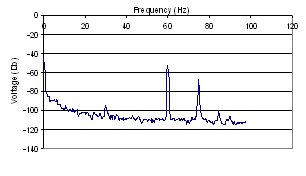
\includegraphics[width=0.5\linewidth]{images/LLSimage019.png}}
        \caption{A plot of data}
        \label{fig:LLSimage019}
    \end{figure}

    \item Now do the same thing, only change the Span to 195 Hz.

    \item As before, to make another data transfer you do not need to restart the program. There are two choices. One, click on the arrow in the upper left corner (note: this arrow only shows up if you have already transferred the data at least once.) Another choice is to choose [ RUN ] from the OPERATE menu option. With either choice you will be asked to chose between [ SCREEN CAPTURE ] or [ MAKE SETTINGS REMOTELY ].

\end{enumerate}


\textbf{This is a Checkpoint: Call over a GSI or Professor and explain what you know of 1/f noise and its origins. Why does it diverge at 0 Hz. Does the sample you took follow a 1/f spectrum? Where does the 60 Hz noise come from (source)? What does changing the span do to our signal? (Think about the sampling time, rate and span in relation to each other) How can you get a better resolution to figure out a more accurate answer of the next question. At what frequency range does flicker noise seem to dominate? Where does it disappear relative to the noise floor (the background noise at high frequencies)? What is happening here? }

\section{Capacitive Coupling Noise}

AC voltages from nearby electronics create stray capacitive effects. Careful design can nearly eliminate capacitive noise.

\subsection{Notes}

\begin{itemize}
    \item \textbf{Frequencies to be wary of:}
    \begin{itemize}
        \item 60/120 Hz and harmonics

        \item AM broadcasts at 0.5 to 2 MHz

        \item CB radio around 30 MHz

        \item FM and TV bands at around 100 MHz

        \item Radar and Microwave around 10 GHz

    \end{itemize}

    \item \textbf{Sources of Capacitive noise}
    \begin{itemize}
        \item Other parts of the circuit in question

        \item Power lines/cords etc.

        \item Automobile ignition systems

        \item Microwave ovens

        \item Electrical discharges

        \item Electric motors

        \item Electromechanical switches and relays

    \end{itemize}

\end{itemize}

\subsection{Exercise I (From Building Scientific Apparatus)}

\href{http://physics111.lib.berkeley.edu/Physics111/Reprints/Apparatus\%20Book/Building-Scientific-Apparatus--Moore.pdf}{\textbf{The Book Scientific Apparatus}} The Table of Contents \href{http://physics111.lib.berkeley.edu/Physics111/Reprints/Apparatus\%20Book/toc.pdf}{\textbf{Table of Contents}}

Estimate the minimum stray capacitance, $C_\text{min}$,needed to induce a 1 m$V_\text{rms}$ voltage across a 1 M$\Omega$ resistor from a 120 $V_\text{rms}$ power line ($f$ = 60 Hz). \emph{Hint: Use the model below:}

\begin{figure}[h]
    \centering
    \href{http://experimentationlab.berkeley.edu/sites/default/files/images/LLSimage022.gif}{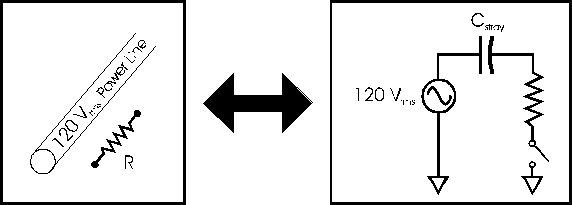
\includegraphics[width=0.5\linewidth]{images/LLSimage022.png}}
    \caption{The model of an equivalent circuit}
    \label{fig:LLSimage022}
\end{figure}

The figure on the left depicts the possible capacitance between a high voltage line and a resistor separated by some arbitrary amount of distance. The figure on the right shows a translation of this image into a circuit (where the stray capacitor can be thought of as the separation in space between the power line and resistor in the first image).

Remember that the current leaving the capacitor is the one entering the resistor. When a constant frequency signal is passing through a capacitor, the capacitor has a fixed impedance = $\frac{1}{2 \pi f C}$. There are two equations and one unknown. Equate the current for both values and solve for C.

Is this a large capacitance? Keep in mind that the capacitance of one foot of RG/58 coaxial cable is 33 pF.

\subsection{Experiment VII}

\emph{Now you get to explore capacitive noise! This is mostly a qualitative experiment in which you play with dangling inputs and see just how much noise can be induced in a typical lab environment. It is at this point that you get to change those annoying 60/120 Hz peaks!}

\begin{enumerate}
    \item Turn on the SR760 FFT and start the \emph{LowLight SR760 Interface} program.

    \item Pick [ MAKE SETTINGS REMOTELY ]

    \item Hook up a coaxial cable to INPUT A of the SR760 and let it lie on the table (unterminated).

    \item Use the default settings of the \emph{LowLight SR760 Interface} program (i.e. SPAN = 1.56 kHz, etc.) and take a data run. Save the data and include it in your lab write-up.

    \item \textbf{What do you see? Explain the existence of the different peaks. Speculate why there are harmonics on the fundamental. Do you see any 1/$f$ noise?}

    \item Let's get a better look at that 60 Hz noise. Take another data run, only this time set the SPAN to 97.5 Hz. Include this data run in your lab write-up, also.

    \item To get an idea as to how much noise is really being induced in the cable, measure and record the height of the peak centered on 60 Hz (you can either do this with the interface program or with the SPIN KNOB on the FFT (make sure you hit the [ MEAS ] button first, though).

    \item Does the orientation of the cable affect the magnitude of the induced noise? Experiment with different orientations of the unshielded cable (e.g. lying flat on the table vs. hanging straight down, etc). \textbf{Explain what you see.}

    \item Now coil the cable up. \textbf{What happens to the 60 Hz peak} (Look at the FFT screen.) Stuff the coiled cable into the brass tube provided. \textbf{Again, what happens to the 60 Hz peak? Measure and record the magnitude of the 60 Hz peak for both cases.} (Use either the FFT or the interface program-see (6) above.)

    \item With the cable stuffed in the brass tube, ground the brass tube (the instrument rack should suffice as a ground). There should be some clips hanging from the ring stand by the computer. \textbf{What happens? Again, measure the height of the peak}. Include in your write-up a plot of the data with the grounded brass tube around the cable.

\end{enumerate}


\textbf{This is a Checkpoint: Compare the magnitudes of the peaks in units of volts (not dBV). Explain why coiling the wire reduces the noise, why shielding the cable reduces it some more, and why grounding the shield reduces it even further.}\\
Now you see why sensitive experiments are usually locked up in a Faraday Cage. Other common ways to eliminate Capacitive noise include:

\begin{itemize}
    \item Using tri-axial cable. Tri-axial cable is basically co-axial cable with an extra metal braid around it.

    \item Removing the annoying noise source

    \item Using low (high) impedance for voltage (current) measurements. \emph{\textbf{***Explain why this works***}}

    \item Keep lines close to ground and away from fringing fields.

\end{itemize}

\section{Microphonic Noise}

\subsection{Exercise II:}

Estimate the magnitude of the Microphonic noise caused by shaking one meter of RG/58 coaxial cable at a frequency of 10 kHz. Assume that:

\begin{itemize}
    \item The cable has 1 V across it and a capacitance of 33pf/foot.

    \item It goes into a scope with a 1 M$\Omega$ input impedance

    \item The shaking causes a change in capacitance ($\delta C$) of 1 pF (does this sound reasonable? What is $\delta C/C$?)

\end{itemize}

\subsection{Experiment VIII}

This experiment is almost completely qualitative. You'll look at some Microphonic noise on the FFT. The source will be a dangling input, which you will shake by hand.

\begin{enumerate}
    \item Turn on the SR760 FFT and start the \emph{\textbf{LowLight SR760 Interface}} program.

    \item Since you'll be providing the Microphonic action (i.e. shaking the cable), you probably won't need to look at the frequency spectrum above 100 Hz-unless you're a super-duper tambourine player. So set the SPAN to 97.5 Hz using the \emph{\textbf{Interface}} program. Also turn LINEAR AVERAGING off, if it is on (you'll want to track the happenings in real time, as the frequency of your shaking will probably vary a little).

    \item Hook up a coaxial cable to INPUT A and let it cable hang still. Using the \emph{\textbf{Interface}} program, take a set of data points. Look at the spectrum. You should see something as in \textbf{Figure \ref{fig:WithoutShakingTheCable}}. Note the 1/$f$ and capacitive noise. Include a copy of these data in your lab write-up.

    \begin{figure}[h]
        \centering
        \href{http://experimentationlab.berkeley.edu/sites/default/files/images/LLSimage025.gif}{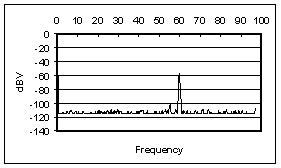
\includegraphics[width=0.5\linewidth]{images/LLSimage025.png}}
        \caption{Without Shaking the Cable}
        \label{fig:WithoutShakingTheCable}
    \end{figure}

    \item Now shake the cable at a semi-constant frequency (\emph{Note: you don't have to go crazy. You're not trying to kill snakes or anything. Just shake it gently}). \textbf{Comment on what happens on the FFT screen.} Using the \emph{\textbf{Interface}} program, take a set of data while shaking the cable. Your data should look something like \textbf{Figure \ref{fig:ShakingTheCable}}.

    \begin{figure}[h]
        \centering
        \href{http://experimentationlab.berkeley.edu/sites/default/files/images/LLSimage026.gif}{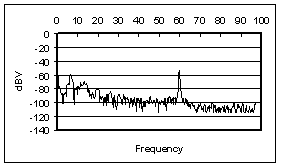
\includegraphics[width=0.5\linewidth]{images/LLSimage026.png}}
        \caption{Shaking the Cable}
        \label{fig:ShakingTheCable}
    \end{figure}

    Notice how large harmonic components appear around the frequency that you're shaking the cable. \textbf{Why are there multiple peaks? Why are they broad?} Notice how a little bit of shaking can produce noise that easily matches the Capacitive pick-up at 60 Hz. Also note how it is harder to isolate non-affected frequencies (i.e. the noise is spread out over a large band of frequencies, not just peaked at 60 Hz or so).

    \item Explore the Microphonic noise effects using different values of the SPAN. You don't need to use the \emph{Interface} program to save these data points. Just adjust the SPAN using the SPIN KNOB on the FFT. \textbf{Comment on anything you find interesting}.

    \item \textbf{List some ways to avoid Microphonic Noise.}

\end{enumerate}

\section{Shot Noise}

\begin{itemize}
    \item It is a form of \emph{white noise}, noise that has the same power density at all frequencies.

    \item At a given frequency, the voltage fluctuations are Gaussian in nature (i.e. if you plotted a histogram of voltage measurements at any specific frequency at a number of equally spaced times, it would be Gaussian in shape).

    \item Note: When using instruments such as the SR830, the bandwidth is given by the ENBW (Effective Noise Bandwidth), specified in the manual (page 3-21 in the SR830 manual). This applies to all forms of Gaussian noise.

\end{itemize}

\subsection{Exercise III}

Calculate the shot noise for the Pin-10DP Pin Diode in units A/$\sqrt{\text{Hz}}$. These units may seem peculiar, but they are in universal use. We really want the power/unit frequency interval, which is the square of the units that are used. Notice how the shot noise increases with increasing signal current. If we wanted to recover our signal better, and our only concern was shot noise, would we want a higher or lower signal current? For what value of the signal current would the signal and shot noise currents be equal?

\emph{At this time, there is no experiment for shot noise.}

\section{Instrument Noise}

When you stop and think about the many resistors and other components inside instruments, it's not surprising that they are also sources of noise. The noise added to the signal is usually proportional to $\sqrt{\triangle f}$, where $\triangle f$ is the bandwidth. To get an idea of how big these noise sources are, refer to:

\begin{itemize}
    \item \emph{\textbf{SR830}} Lock-In Manual, p. (3-17). Input noise $\sim$ 5 n$V_\text{rms}/\sqrt{\text{Hz}}$

    \item \emph{\textbf{SR570}} Current Preamplifier Manual, p. vii. Input noise ranges from 150 pA/$\sqrt{\text{Hz}}$ to 5 fA/$\sqrt{\text{Hz}}$. \emph{Note: to get this as an output noise in $V_\text{rms}$, divide it by the SENSITIVITY.}
\end{itemize}

\begin{enumerate}
    \item Note: When using instruments such as the \emph{\textbf{SR830}}, the bandwidth is given by the ENBW (Effective Noise Bandwidth), specified in the manual (page 3-11 in the \emph{\textbf{SR830}} manual). This applies to all forms of Gaussian noise.
\end{enumerate}

\noindent\emph{There is no exercise or experiment for instrument noise.}

\section{Johnson Noise}

(Read p. 458 of \emph{Building Scientific Apparatus})

\begin{itemize}
    \item It arises from statistical fluctuations in electron motion in a resistor at finite temperature. It can be derived using ideas based on Black Body radiation. For a derivation, see \emph{Thermal Physics} by Kittel, p. 98.

    \item At a given frequency, the voltage fluctuations are Gaussian in nature (i.e. if you plotted a histogram of voltage measurements, it would be Gaussian)

    \item It is \emph{white noise}-i.e. exists at all frequencies with the same magnitude. So the more frequencies you sample, the more Johnson noise you get.

    \item Johnson noise also presents itself in the form of a current:
    \[
    I_\text{J, rms}^2 = \frac{V_\text{J, rms}^2}{R_\text{source}^2} = \frac{4kT\triangle f}{R_\text{source}}
    \]

    \item It is independent of material-everything with the same resistance has the same Johnson noise.

    \item The units V/$\sqrt{\text{Hz}}$ and A/$\sqrt{\text{Hz}}$ appear a lot in the noise business (usually in the context of \emph{white noise}). In order to actually get a value for the noise, you'll need to multiply the quoted value by $\sqrt{\triangle f_b}$, where $\triangle f_b$ is the bandwidth of your measurement.

    \item Note: When using instruments such as the SR830, the bandwidth is given by the ENBW (Effective Noise Bandwidth), specified in the manual (page 3-11 in the SR830 manual). This applies to all forms of Gaussian noise.

\end{itemize}

\subsection{Exercise IV}

Calculate the Johnson current noise for the Pin-10DP Pin diode. Express your answer in V/$\sqrt{\text{Hz}}$. Would you want a current signal to come from a high impedance source or a low impedance source if you were concerned about Johnson noise? What if it were a voltage source? Why?

\subsection{Experiment IX}

\subsubsection{Notes}

In this experiment, you will use the SR830 Lock-In to measure Johnson noise and its dependence on $ R_\text{source} $ and $ \triangle f_b $ by hooking up various resistors across the input of the SR830. \emph{Note: Compared to the previous small experiments, this is rather involved.}\\

\noindent\textbf{A former student makes these comments:}

\noindent\emph{Reasons for using the spectral analyzer are:}

\begin{itemize}
    \item You get a picture of what the entire noise spectrum looks like, instead of just some number. You aren't taking a ``shot in the dark'' and can avoid hitting a noise peak. There are other peaks besides the 60 Hz harmonics.

    \item The SR760 can tell you the noise power at a point as well as within a bandwidth.

    \item You can press a few buttons and get an answer really fast.

    \item You get a better ``feel'' of whether or not your answer makes sense.

    \item You get better answers because the scope takes more averages.

    \item The Lock-in Lab-View program occasionally gives totally wacky values.
\end{itemize}

\noindent\emph{Reasons for using the Lock-in to take measurements after using the spectrum analyzer to take a look at the noise are:}

\begin{itemize}
    \item You get to use some of the ``effective bandwidth'' stuff you learned earlier.

    \item There is slightly more physics involved, as you can actually see some of the voltage fluctuations.

\end{itemize}

\subsubsection{Procedure}

\begin{enumerate}
    \item Turn on the SR830 Lock-In and start the \emph{SR830 Lock-In Interface} program.

    \item Via a coaxial cable, hook up a pair of clips to the INPUT A/I of the Lock-In. Make sure that the cable is short and stiff. \textbf{Why is this important?}

    \item Unplug any input to the REF IN. You will use the Lock-In's internal oscillator as a reference.

    \item Since you're using the internal oscillator, you'll have to choose and set the frequency of oscillation manually:
    \begin{enumerate}
        \item Depress the [ SOURCE ] button by the SPIN KNOB until INTERNAL is chosen. This tells the SR830 that you'll be using the internal oscillator as a reference signal.

        \item Depress the [ FREQ ] button above the SPIN KNOB. This will allow you to choose the frequency of oscillation.

        \item Turn the SPIN KNOB until the desired frequency set. Make sure to choose the frequency wisely so as to eliminate as much non-Johnson noise as possible. \textbf{Record your frequency choice and reasons for choosing it.}

    \end{enumerate}

    \item Connect a 100 k$\Omega$ resistor across the clips. Set the TIME CONSTANT to 30 ms and adjust the SENSITIVITY appropriately. Also, select the highest SLOP/OCT rolloff, 24 dB. Use the ``Low noise'' setting and NOT ``High reserve''.

    \item Input the following settings on the \emph{\textbf{Interface}} program:
    \begin{enumerate}
        \item Data Run and Save Options

    \begin{enumerate}
        \item NUMBER OF RUNS: 7 (the more measurements, the better)

        \item SAVE DATA?: Yes (box checked) (include in your lab write-up the analyzed data in table format and a plot of the raw data)

        \item SAVE DATA TO: \emph{You decide}. For your purposes, one file would probably be just fine. It is recommended that you include information relevant to the measurement, such as the value of the resistor, and the SLOP/OCT rolloff.

    \end{enumerate}

        \item Data Acquisition Options

        \begin{enumerate}
            \item GPIB ADDRESS: 8 (That's where the SR830 lives in the wonderful world of GPIB and you do not change it.)

            \item SAMPLE MODE: BEST CHOICE is recommended. \emph{Note: Sometimes taking more than 1200 data points doesn't work. If this happens, consider using the }BEST CHOICE\emph{ mode while selecting the }TIME CONSTANT\emph{. This way, the computer will choose an appropriate }SAMPLE RATE\emph{ for you. Then switch to }CUSTOM\emph{ mode and adjust }\emph{the }SPAN\emph{ so as to reduce the} TOTAL NUMBER OF DATA POINTS\emph{ below 1200.}

            \item TIME CONSTANT: 30 ms

            \item Press [ START ].

        \end{enumerate}

    \end{enumerate}

    \item Let the \emph{\textbf{Interface}} program take the data for you. Watch to make sure that you're getting good data. Things to look out for:
    \begin{enumerate}
        \item \textbf{All of your data are zero or some other constant value}. A possible problem is that the Sensitivity isn't adjusted correctly or that it is overloaded.

        \item \textbf{Some of your data are zero}. Perhaps you need to reduce the TOTAL NUMBER OF DATA POINTS below 1200.

        \item \textbf{The data look very ``spiky''. WHY IS THIS A PROBLEM (this is a question for you to answer)?} The SAMPLE RATE is probably too low. Increase it. Your data should look rather rounded and contain as many ``periods'' as possible. See \textbf{Figure \ref{fig:DataNotSpikyAndHavePeriods}}.

        \begin{figure}[h]
            \centering
            \href{http://experimentationlab.berkeley.edu/sites/default/files/images/LLSimage040.gif}{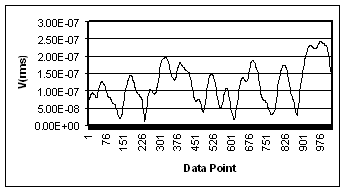
\includegraphics[width=0.5\linewidth]{images/LLSimage040.png}}
            \caption{The data aren't ``spiky'' and have quite a few ``periods''}
            \label{fig:DataNotSpikyAndHavePeriods}
        \end{figure}
    
        \item The data don't have many ``periods.'' \textbf{WHY IS THIS A PROBLEM (this is a question for you to answer)?} The SAMPLE RATE may be too high. Decrease it, keeping in mind the tradeoff with ``spikiness'', above.

    \end{enumerate}
    
    \item It should take just a minute or two for the \emph{\textbf{Interface}} program to collect, analyze, and save the data. Open the file ``\textbf{[base file path] Analyzed Data (T= [time constant] ).xls}'' in Excel. You should see something like the following (note, this sample only represents 3 data runs using a resistor that was not 100 k$\Omega$):
    \begin{center}
    \begin{tabular}{l|l|l}
        $\langle R \rangle$ & $\langle dR^2 \rangle^{1/2}$ & $\langle dR \rangle$ \\\hline
        1.18E-07 & 5.73E-08 & 4.79E-08 \\\hline
        1.64E-07 & 6.81E-08 & 5.19E-08 \\\hline
        1.52E-07 & 6.71E-08 & 5.54E-08
    \end{tabular}
    \end{center}

    \item Find the average value of your ${\langle \triangle R^2 \rangle}^{1/2}$ measurements and compare it to the theoretical value (remember: $R$ stands for magnitude of the measurement made by the Lock-In). Is your measurement off by about a factor of $\sqrt{2}$? \textbf{If it is, why}?
    
    \item Repeat the above procedure for TIME CONSTANT values of 100 msec., 300 msec., 1 sec., and 3 sec. \emph{Note: taking data at high TIME CONSTANT values will take a long time. You can let it run overnight or while you go to get lunch, if you want.}
    
    \item To see how the Johnson Noise varies with resistance, repeat the above procedure using a 10 k$\Omega$ resistor.

\end{enumerate}

\textbf{This is a Checkpoint: Call over a Professor or GSI and discuss what you have learned from the different noises surrounding this experiment. Compile all your data and plot them.  How well do they agree with theory (remember to calculate $\triangle f$ using the ENBW specified on page 3-11 of the SR830 manual)? What would you expect for such a crude experiment? Remember to account for the Lock-In input noise: $V_\text{Tot, noise}^2 = V_J^2 + V_\text{Input}^2$.}

\subsubsection{General comments about getting low-noise signals}

There are three techniques that you can use to reduce the amount of noise in your signal. The first is using shorter cables. The shortest ``cable'' is a male BNC barrel connector. The second is using "differential inputs, which you can read about on pages 3 to 19 in the SR830 manual. In brief, you can use two cables to measure the signal so that the noise common in both cables cancels out. These two techniques reduce the external noise. The third is running your experiment at low temperatures. After finishing this section, you might dunk your resistor in liquid nitrogen to see how it affects the intrinsic (Johnson) noise of the resistor. Just be sure to note $R$ as a function of $T$, and don't get the inputs on the equipment cold, or water could condense on them.

\section{Experimental Setup}

We are now ready to apply what we have learned. Our goal is to measure the light output of an LED using the 10DP Pin Diode. We'll complicate things by taking this measurement with a lot of background noise sources such as overhead room lights.

How should we go about taking such a measurement? We learned that if we can modulate our light source at a known frequency, we can use the SR830 Lock-In to recover any signal at that frequency. To do just this, we chop our light signal with a chopper wheel. In essence, we are turning our D.C. signal into an oscillating signal. In a typical setting, the chopper wheel slits are much larger than the light source-making a square wave. In this experiment, however, the chopper slits are just about the same size as the LED, so that we'll be stuck with something closer to a triangular wave. See \textbf{Figure \ref{fig:PowerVsTime}}:

\begin{figure}[h]
    \centering
    \href{http://experimentationlab.berkeley.edu/sites/default/files/images/LLSimage044.gif}{
\includegraphics[width=0.5\linewidth]{images/LLSimage044.png}}
    \caption{The Power Plot}
    \label{fig:PowerVsTime}
\end{figure}

\noindent Using this technique, we can recover the LED signal even though there may be a lot of other light sources around.

\section{Block Diagram I}

\begin{figure}[h]
    \centering
    \href{http://experimentationlab.berkeley.edu/sites/default/files/images/LLSimage045.gif}{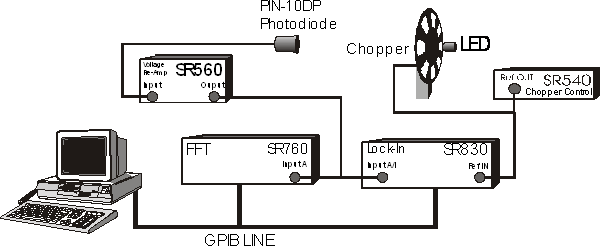
\includegraphics[width=0.5\linewidth]{images/LLSimage045.png}}
    \caption{Block Diagram 1}
    \label{fig:BlockDiagramI}
\end{figure}

Shown above in \textbf{Figure \ref{fig:BlockDiagramI}} is a block diagram for the experiment. The LED signal is chopped by the chopper, whose frequency is set by the SR540 Chopper Controller. The chopped signal is detected by the PIN-10DP photodiode, which sends a current signal to the SR570 Low-Noise Current Preamplifier. The SR570 amplifies, filters, and measures the input current signal and you convert it to an output voltage signal. The voltage signal is then sent to the SR760 FFT and the SR830 Lock-In Amplifier. The reference signal for the Lock-In is provided by the SR540. Finally, the computer gathers and analyzes the data.

You may be asking yourself, ``why do we need to use the SR570? It just adds a bunch of noise to our signal! It can't just be that the SR570 will convert the current signal to a voltage! I read that the Lock-In can accept either a voltage or a current. So what is the purpose of the SR570?''

Well, it's true that the SR830 will accept an input current. If you read carefully, you'll notice that the maximum input DC current is 10 $\mu$A and the maximum input AC current is 1.4 $\mu$A. \textbf{Under our operating conditions, what is a typical current output of the Pin-10DP (measure it)?}

If the current is too large, we will have to use the SR570. First let us see whether or not just converting the current signal into a voltage signal will help us any (the SR830 may have different overload tolerances for voltages than for currents). Now, the SR830 will overload for voltage inputs greater than 1.4 Vpk. \textbf{On the lowest usable sensitivity of the SR570 (determined in Exercise V), what output voltage would result from an input current of 10 $\mu$A (enough current to overload the SR830)? How much bigger/smaller can/should our current signal be if we use the SR570 at this sensitivity (and without filtering) before sending it to the SR830 Lock-In?} If you find that we haven't gained anything by simply converting the current into a signal, consider this: a lot of the signal from the 10DP is noise. If we could eliminate most of that noise before we sent it into the SR830, it would be to our advantage. That's where using the filtering options on the SR570 comes in. \textbf{What are some frequencies that we would like to attenuate?}

\subsection{Exercise V}

If we were using Block Diagram I (textbf{Figure \ref{fig:BlockDiagramI}}) for our experiment, determine the minimum sensitivity we should set on the SR570. Use the table in the SR570 Operation manual to determine the minimum amount of noise (in A/$\sqrt{\text{Hz}}$) that will be added to our signal by the SR570. Compare that to the Johnson current noise and Shot noise of the Pin-10DP in normal operating mode (hint: you'll need to know the resistance of the Pin-10DP).

\subsection{Experiment X}

\textbf{In this little experiment, you'll pretend to be an astronomer trying to find and measure the signal from a pulsar.}

\begin{enumerate}
    \item Choose the Experimental Set-Up in \textbf{Block Diagram I}.

    \item Hook up and turn on the equipment as shown in the \textbf{Block Diagram I} (note that the switch in Block Diagram I is purely symbolic.
    \begin{enumerate}
        \item Connect DP-10 Pin Diode to SR570 Input

        \item Connect output of SR570 to the A Input of SR760 and A/I Input of SR830

        \item You will manually disconnect and reconnect the BNC). However, don't hook up the reference signal to the REF IN port on the SR830. After all, astronomers don't have such a luxury. Make sure the reference on the SR830 is set to INTERNAL.
    \end{enumerate}

    \item Turn on SR760, SR570, and SR830

    \item Turn on AC Power to the top Remote Control Box (RCB). This box remotely controls the RED LED and the Chopper.

    \item Switch the VARIAC VOLTAGE of the RCB to LAMP and 0-5 V ADJUST to ON (dial can be set around 7).

    \item Make appropriate choices for the sensitivities of the SR830 and the SR570. You may notice that the SR830 sensitivity overloads for no apparent reason. To fix this, you may need to attach the cone to the 10DP Pin Diode (as mentioned above), or use the ``high Reserve'' setting on the Lock-in. To get the best signal-to-noise ratio, think carefully about what the output of the diode is like, and where to put the gain and filtering stages. You can get a fairly good ratio by fiddling around with the settings.

    \item Look at the signal on the FFT.

    \item Set the SPAN of FFT to 1.56kHz.

    \item Try to identify which peak represents the ``pulsar'' by using your knowledge of noise sources to eliminate the other peaks. Turn the light off to see if the signal disappears.

    \item Vary the VARIAC VOLTAGE of the \href{http://experimentationlab.berkeley.edu/node/98}{\textbf{Remote Control Box}} and the 0-5 V ADJUST to see the frequency and voltage change. Variac Voltage changes the amplitude of the white light only and the 0-5 V Adjust changes the frequency of the chopper.

    \item Now feed the signal to the SR830 and set the reference frequency to what you decided belongs to the ``pulsar.''

    \item Scan the reference frequency in order to maximize the signal. Keep in mind how the response time of the SR830 depends on your choice of TIME CONSTANT and ROLLOFF.

    \item So what frequency did you find the ``pulsar'' to be flashing at? Is that the correct frequency? To determine the correct frequency, hook up the reference signal from the chopper to the REF IN on the SR830 and set the reference source to external (i.e. not INTERNAL or UNLOCK). How close were you?
\end{enumerate}

\subsection{Experiment XI}

\textbf{In this experiment, you'll actually measure the signal from the LED.}

\begin{enumerate}
    \item Hook up and turn on the equipment as shown in \textbf{Block Diagram I} (this is the same set up as in the \textbf{Experiment X}). Turn on the \textbf{RED} LED and the chopper using the remote box affixed to the instrument rack (See \href{http://experimentationlab.berkeley.edu/node/98}{\textbf{Appendix C: the Remote Control Box}}). \emph{\textbf{DO NOT}} fiddle with the chopper control box in the corner of the room. You can read the chopper frequency using the Lock-In (make sure that the reference signal is not set to INTERNAL).

    \item Make appropriate choices for the sensitivities of the SR830 and the SR570. You may notice that the SR830 sensitivity overloads for no apparent reason. To fix this, make sure the cone is attached to the 10DP Pin Diode.

    \item Adjust the photodiode and the cone so that you receive a maximum signal on the SR830 (you may want to adjust the time constant to make alignment easier).

    \item Look at the spectrum of the signal on the FFT. Use either the \emph{\textbf{Interface}} program or the controls on the FFT. Make sure that the SPAN includes the frequency of the signal. Do you see the signal? Play with the FILTER TYPE on the SR570 and see what happens to the spectrum.

    \item Adjust the frequency of the chopper signal appropriately so as to eliminate external noise sources as much as possible. You may want to turn on the halogen lamp during this process. \textbf{State how you avoided the following noise sources by adjusting the frequency (if it is possible): 1/$f$ noise, Johnson noise, Microphonic noise, 60/120 Hz noise, shot noise, instrument input noise}.

    \item Use the \emph{\textbf{LowLight SR760 FFT Interface}} to gather some sample data showing which frequency you used (make sure the LED/halogen lamp peak is clearly visible). Include a plot of it in your write-up.

    \item We'll now use the Lock-In to measure the LED signal. Use the \emph{\textbf{LowLight SR830 Lock-In Interface}} program to take several measurements of the input signal (remember to turn off the halogen lamp if it is on). Choose your TIME CONSTANT and time constant rolloff (SLOP/OCT) appropriately so as to get as good a signal as possible (suggestions: $\tau$ = 30 sec at 24 dB).\textbf{State how your choice of time constant and rolloff can/cannot reduce the noise sources listed in 6)}. If you want, let the data run go overnight. Be sure to do several runs.

    \item Now estimate the power from the diode and compare it to your measurement. See the next section about how to interpret your data and \href{http://experimentationlab.berkeley.edu/node/100}{\textbf{Appendix E}} about how to estimate the actual power emitted by the LED.

\end{enumerate}

\section{Interpreting the Data}

Estimate all the errors that should have appeared in your data and see if they correspond to the observed $\langle \triangle R^2 \rangle^{1/2}$. Take into account all the sources of noise discussed so far (don't forget the instrument noise).

Now determine how well the measured value of the signal, $\langle  R \rangle$, correlates to the power output of the diode. Some things to keep in mind/think about:

\begin{enumerate}
    \item \textbf{What is it that the Lock-In is measuring? Is it the DC power of the LED? Is it the amplitude of a triangle wave (if it is, how does this relate to the DC output of the LED?)? Determine what you are actually measuring.}

    \item \textbf{How does the 10DP photodiode convert the incident power to a current? According to the specifications, the conversion is roughly 0.35 A/W. So if one milliwatt of light were incident on the diode, you would expect 0.35 x 10-3 A to come out of the diode. }

    \item \textbf{How does the SR570 convert this current into a signal? (This is easy. Answer it even if you didn't use it to measure your signal).}

\end{enumerate}

So now you have traced everything back to the photodiode. \textbf{Based on your data, what would be the DC power incident on the photodiode from the LED if the chopper were not there?}

Now that we know this, it's time to correlate this value to the actual DC power output of the LED. To do this, we must determine, given the LED power output, how much power would hit the photodiode. This is basically just the integral over the photodiode's surface:
\begin{equation}
    P_\text{photodiode} = \int_\text{photodiode's surface} I(\vec{r}) \,dA
\end{equation}
where $I(\vec{r})$ is the intensity of the light from the LED as a function of position. All we need to know is $I(\vec{r})$. Looking at the data sheet, it seems reasonable to make the approximation that $I(\vec{r})$ has the form
\begin{equation}
    C \frac{\cos^2{\theta}}{r^2}
\end{equation}
where $C$ depends only on the power output of the LED, $\theta$ is the angle listed on the data sheet, and $r$ is the distance from the LED (so that in polar coordinates, the LED would be oriented along the $z$-axis).

Shown in \textbf{Figure \ref{fig:RadiationProfile}} is the actual radiation profile of the LED and the $\cos^2\theta$ approximation (as a function of the angle $\theta$). Note that using this approximation, we will be \emph{overestimating} the actual power output of the diode, as the area contained in the approximate distribution is larger than that contained in the actual profile. \textbf{About how much of an error do you estimate that this approximation will introduce to our measurement?}


\begin{figure}[h]
    \centering
    \href{http://experimentationlab.berkeley.edu/sites/default/files/images/395px-Diode_Distribution.png}{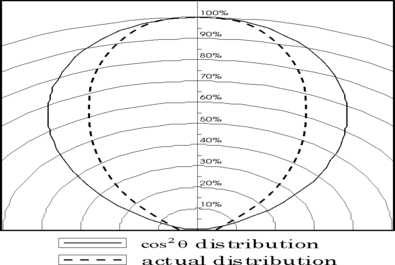
\includegraphics[width=0.5\linewidth]{images/395px-Diode_Distribution.png}}
    \caption{The Diode Distribution}
    \label{fig:RadiationProfile}
\end{figure}

Now, we can find the exact form of C by noting that the total power output of the diode, P, satisfies
\begin{equation}
    P = \int_0^{\pi}\, d\theta \int_0^{2\pi}I(\vec{r})r^2\sin{\theta}\, d\phi
    = 2\pi\int_0^{\frac{\pi}{2}}C\cos^2{\theta}\sin{\theta}\, d\theta
    = \frac{2\pi}{3}C
\end{equation}
So that
\begin{equation}
    C = \frac{3P}{2\pi}
\end{equation}
Note that the bounds in the $d\theta$ integral changed from $(0\rightarrow\pi)$ to $(0\rightarrow\frac{\pi}{2})$. \textbf{Explain why.}

So now we know an approximate form for $I(\vec{r})$. In calculating the power that would fall upon the photodiode, we can make another approximation based on the orientation of the photodiode: $P_\text{photodiode} \approx I(\theta = 0, r) \times$ Area of Photodiode

\textbf{Justify this approximation.}

Now, using the Control box (see \href{http://experimentationlab.berkeley.edu/node/98}{\textbf{Appendix C: the Remote Control Box}}), determine P, the power output of the LED. To get an idea of the efficiency of the LED, you should refer to \href{http://experimentationlab.berkeley.edu/node/100}{\textbf{Appendix E: Interpreting the Data Sheet for the LED}}

Once you do that, determine $P_\text{photodiode}$ and compare this to the value that you measured. How well do they agree? To within a factor of 2? We really couldn't hope for much more than that given our somewhat crude approximations.

\begin{itemize}
    \item Last day of the experiment please fill out the \href{\ExperimentEvaluation}{\textbf{Experiment Evaluation}}

\end{itemize}

\section{References}
\label{sec:References}

\begin{enumerate}
    \item \href{http://physics111.lib.berkeley.edu/Physics111/Equipment\_Manuals/LLS/indexequipLLS.html}{\textbf{Equipment\_Manuals}}

    \item Noise in Electronic Devices and Systems by Buckingham (you will need to make an \href{http://oskicat.berkeley.edu/screens/help\_borrowing.html#nrlfrequest}{\textbf{NRLF request}} to get this book)

    \item Electronic Noise and Fluctuations in Solids by Kogan (Located in the Physics and Astronomy Library, call number is \href{http://oskicat.berkeley.edu/search\~S1?/cQC176.8.E4+K864+1996/cqc++176.8+e4+k864+1996/-3,-1,,B/browse}{\textbf{QC176.8.E4 K864 1996}}) \href{http://physics111.lib.berkeley.edu/Physics111/Reprints/LLS/Electronic\%20Noise\%20and\%20Fluctuations\%20in\%20Solids_Kogan.pdf}{\textbf{Searchable PDF version}}

\end{enumerate}

\noindent Other reprints and reference materials can be found on the \href{http://physics111.lib.berkeley.edu/Physics111/Reprints/LLS/LLS\_index.html}{\textbf{Physics 111 Library Site}}

\end{document}
